\documentclass[twoside]{book}

% Packages required by doxygen
\usepackage{fixltx2e}
\usepackage{calc}
\usepackage{doxygen}
\usepackage[export]{adjustbox} % also loads graphicx
\usepackage{graphicx}
\usepackage[utf8]{inputenc}
\usepackage{makeidx}
\usepackage{multicol}
\usepackage{multirow}
\PassOptionsToPackage{warn}{textcomp}
\usepackage{textcomp}
\usepackage[nointegrals]{wasysym}
\usepackage[table]{xcolor}

% Font selection
\usepackage[T1]{fontenc}
\usepackage[scaled=.90]{helvet}
\usepackage{courier}
\usepackage{amssymb}
\usepackage{sectsty}
\renewcommand{\familydefault}{\sfdefault}
\allsectionsfont{%
  \fontseries{bc}\selectfont%
  \color{darkgray}%
}
\renewcommand{\DoxyLabelFont}{%
  \fontseries{bc}\selectfont%
  \color{darkgray}%
}
\newcommand{\+}{\discretionary{\mbox{\scriptsize$\hookleftarrow$}}{}{}}

% Page & text layout
\usepackage{geometry}
\geometry{%
  a4paper,%
  top=2.5cm,%
  bottom=2.5cm,%
  left=2.5cm,%
  right=2.5cm%
}
\tolerance=750
\hfuzz=15pt
\hbadness=750
\setlength{\emergencystretch}{15pt}
\setlength{\parindent}{0cm}
\setlength{\parskip}{3ex plus 2ex minus 2ex}
\makeatletter
\renewcommand{\paragraph}{%
  \@startsection{paragraph}{4}{0ex}{-1.0ex}{1.0ex}{%
    \normalfont\normalsize\bfseries\SS@parafont%
  }%
}
\renewcommand{\subparagraph}{%
  \@startsection{subparagraph}{5}{0ex}{-1.0ex}{1.0ex}{%
    \normalfont\normalsize\bfseries\SS@subparafont%
  }%
}
\makeatother

% Headers & footers
\usepackage{fancyhdr}
\pagestyle{fancyplain}
\fancyhead[LE]{\fancyplain{}{\bfseries\thepage}}
\fancyhead[CE]{\fancyplain{}{}}
\fancyhead[RE]{\fancyplain{}{\bfseries\leftmark}}
\fancyhead[LO]{\fancyplain{}{\bfseries\rightmark}}
\fancyhead[CO]{\fancyplain{}{}}
\fancyhead[RO]{\fancyplain{}{\bfseries\thepage}}
\fancyfoot[LE]{\fancyplain{}{}}
\fancyfoot[CE]{\fancyplain{}{}}
\fancyfoot[RE]{\fancyplain{}{\bfseries\scriptsize Generated by Doxygen }}
\fancyfoot[LO]{\fancyplain{}{\bfseries\scriptsize Generated by Doxygen }}
\fancyfoot[CO]{\fancyplain{}{}}
\fancyfoot[RO]{\fancyplain{}{}}
\renewcommand{\footrulewidth}{0.4pt}
\renewcommand{\chaptermark}[1]{%
  \markboth{#1}{}%
}
\renewcommand{\sectionmark}[1]{%
  \markright{\thesection\ #1}%
}

% Indices & bibliography
\usepackage{natbib}
\usepackage[titles]{tocloft}
\setcounter{tocdepth}{3}
\setcounter{secnumdepth}{5}
\makeindex

% Hyperlinks (required, but should be loaded last)
\usepackage{ifpdf}
\ifpdf
  \usepackage[pdftex,pagebackref=true]{hyperref}
\else
  \usepackage[ps2pdf,pagebackref=true]{hyperref}
\fi
\hypersetup{%
  colorlinks=true,%
  linkcolor=blue,%
  citecolor=blue,%
  unicode%
}

% Custom commands
\newcommand{\clearemptydoublepage}{%
  \newpage{\pagestyle{empty}\cleardoublepage}%
}

\usepackage{caption}
\captionsetup{labelsep=space,justification=centering,font={bf},singlelinecheck=off,skip=4pt,position=top}

%===== C O N T E N T S =====

\begin{document}

% Titlepage & ToC
\hypersetup{pageanchor=false,
             bookmarksnumbered=true,
             pdfencoding=unicode
            }
\pagenumbering{alph}
\begin{titlepage}
\vspace*{7cm}
\begin{center}%
{\Large C\+B\+R\+A\+PI }\\
\vspace*{1cm}
{\large Generated by Doxygen 1.8.12}\\
\end{center}
\end{titlepage}
\clearemptydoublepage
\pagenumbering{roman}
\tableofcontents
\clearemptydoublepage
\pagenumbering{arabic}
\hypersetup{pageanchor=true}

%--- Begin generated contents ---
\chapter{Hierarchical Index}
\section{Class Hierarchy}
This inheritance list is sorted roughly, but not completely, alphabetically\+:\begin{DoxyCompactList}
\item \contentsline{section}{Abstract\+Feature}{\pageref{class_abstract_feature}}{}
\begin{DoxyCompactList}
\item \contentsline{section}{Case\+Feature}{\pageref{class_case_feature}}{}
\end{DoxyCompactList}
\item \contentsline{section}{Abstract\+Global\+Similarity}{\pageref{class_abstract_global_similarity}}{}
\begin{DoxyCompactList}
\item \contentsline{section}{Euclidean\+Distance}{\pageref{class_euclidean_distance}}{}
\end{DoxyCompactList}
\item \contentsline{section}{Abstract\+Local\+Similarity}{\pageref{class_abstract_local_similarity}}{}
\begin{DoxyCompactList}
\item \contentsline{section}{Equals}{\pageref{class_equals}}{}
\item \contentsline{section}{Linear\+Function}{\pageref{class_linear_function}}{}
\end{DoxyCompactList}
\item \contentsline{section}{Case}{\pageref{class_case}}{}
\item \contentsline{section}{Case\+Base\+Connector}{\pageref{class_case_base_connector}}{}
\item \contentsline{section}{C\+B\+R\+A\+PI}{\pageref{class_c_b_r_a_p_i}}{}
\item \contentsline{section}{Consult\+Params}{\pageref{class_consult_params}}{}
\item \contentsline{section}{Consult\+Structure}{\pageref{class_consult_structure}}{}
\item \contentsline{section}{Result}{\pageref{class_result}}{}
\item \contentsline{section}{Search}{\pageref{class_search}}{}
\end{DoxyCompactList}

\chapter{Class Index}
\section{Class List}
Here are the classes, structs, unions and interfaces with brief descriptions\+:\begin{DoxyCompactList}
\item\contentsline{section}{\hyperlink{class_abstract_feature}{Abstract\+Feature} \\*Classe abstrata que representa a estrutura básica de um atributo. }{\pageref{class_abstract_feature}}{}
\item\contentsline{section}{\hyperlink{class_abstract_global_similarity}{Abstract\+Global\+Similarity} \\*Classe abstrata que representa uma medida de similaridade global que será implementada na biblioteca C\+BR. }{\pageref{class_abstract_global_similarity}}{}
\item\contentsline{section}{\hyperlink{class_abstract_local_similarity}{Abstract\+Local\+Similarity} \\*Classe abstrata que representa uma medida de similaridade local que será implementada na biblioteca C\+BR. }{\pageref{class_abstract_local_similarity}}{}
\item\contentsline{section}{\hyperlink{class_case}{Case} \\*Classe que representa um caso que compõem a base de casos. Composta por um identificador do caso e sua descrição do problema e solução. }{\pageref{class_case}}{}
\item\contentsline{section}{\hyperlink{class_case_base_connector}{Case\+Base\+Connector} \\*Classe resposável por fazer a conexão entre a biblioteca C\+BR e a base de casos. }{\pageref{class_case_base_connector}}{}
\item\contentsline{section}{\hyperlink{class_case_feature}{Case\+Feature} \\*Classe que representa um atributo presente na descrição do problema ou solução de um caso. }{\pageref{class_case_feature}}{}
\item\contentsline{section}{\hyperlink{class_c_b_r_a_p_i}{C\+B\+R\+A\+PI} \\*Classe que deve ser instanciada para ser possível utilizar a biblioteca C\+BR. }{\pageref{class_c_b_r_a_p_i}}{}
\item\contentsline{section}{\hyperlink{class_consult_params}{Consult\+Params} \\*Classe que contém os parâmetros da consulta que serão utilizados para a análise de similaridade entre dois casos. }{\pageref{class_consult_params}}{}
\item\contentsline{section}{\hyperlink{class_consult_structure}{Consult\+Structure} \\*Classe que contém a estrutura de consulta que será utilizada na análise de similaridade entre os casos. }{\pageref{class_consult_structure}}{}
\item\contentsline{section}{\hyperlink{class_equals}{Equals} \\*Classe utilizada como função de similaridade local na qual compara se dois atributos são iguais. }{\pageref{class_equals}}{}
\item\contentsline{section}{\hyperlink{class_euclidean_distance}{Euclidean\+Distance} \\*Classe que utiliza da função da Distância Euclidiana para calcular a similaridade global entre dois casos. }{\pageref{class_euclidean_distance}}{}
\item\contentsline{section}{\hyperlink{class_linear_function}{Linear\+Function} \\*Classe que utilizar uma função linear para calcular a similaridade local entre dois atributos do caso. }{\pageref{class_linear_function}}{}
\item\contentsline{section}{\hyperlink{class_result}{Result} \\*Classe que representa o resultado da consulta realizada na biblioteca C\+BR. }{\pageref{class_result}}{}
\item\contentsline{section}{\hyperlink{class_search}{Search} \\*Classe responsável por realizar o matching entre o caso de consulta e todos os casos da base de casos. }{\pageref{class_search}}{}
\end{DoxyCompactList}

\chapter{File Index}
\section{File List}
Here is a list of all files with brief descriptions\+:\begin{DoxyCompactList}
\item\contentsline{section}{Abstract\+Classes/\hyperlink{_abstract_feature_8cs}{Abstract\+Feature.\+cs} }{\pageref{_abstract_feature_8cs}}{}
\item\contentsline{section}{Abstract\+Classes/\hyperlink{_abstract_global_similarity_8cs}{Abstract\+Global\+Similarity.\+cs} }{\pageref{_abstract_global_similarity_8cs}}{}
\item\contentsline{section}{Abstract\+Classes/\hyperlink{_abstract_local_similarity_8cs}{Abstract\+Local\+Similarity.\+cs} }{\pageref{_abstract_local_similarity_8cs}}{}
\item\contentsline{section}{Core/\hyperlink{_case_8cs}{Case.\+cs} }{\pageref{_case_8cs}}{}
\item\contentsline{section}{Core/\hyperlink{_case_base_connector_8cs}{Case\+Base\+Connector.\+cs} }{\pageref{_case_base_connector_8cs}}{}
\item\contentsline{section}{Core/\hyperlink{_case_feature_8cs}{Case\+Feature.\+cs} }{\pageref{_case_feature_8cs}}{}
\item\contentsline{section}{Core/\hyperlink{_c_b_r_a_p_i_8cs}{C\+B\+R\+A\+P\+I.\+cs} }{\pageref{_c_b_r_a_p_i_8cs}}{}
\item\contentsline{section}{Core/\hyperlink{_consult_params_8cs}{Consult\+Params.\+cs} }{\pageref{_consult_params_8cs}}{}
\item\contentsline{section}{Core/\hyperlink{_consult_structure_8cs}{Consult\+Structure.\+cs} }{\pageref{_consult_structure_8cs}}{}
\item\contentsline{section}{Core/\hyperlink{_result_8cs}{Result.\+cs} }{\pageref{_result_8cs}}{}
\item\contentsline{section}{Core/\hyperlink{_search_8cs}{Search.\+cs} }{\pageref{_search_8cs}}{}
\item\contentsline{section}{Similarity\+Measures/\+Global\+Similarities/\hyperlink{_euclidean_distance_8cs}{Euclidean\+Distance.\+cs} }{\pageref{_euclidean_distance_8cs}}{}
\item\contentsline{section}{Similarity\+Measures/\+Local\+Similarities/\hyperlink{_equals_8cs}{Equals.\+cs} }{\pageref{_equals_8cs}}{}
\item\contentsline{section}{Similarity\+Measures/\+Local\+Similarities/\hyperlink{_linear_function_8cs}{Linear\+Function.\+cs} }{\pageref{_linear_function_8cs}}{}
\end{DoxyCompactList}

\chapter{Class Documentation}
\hypertarget{class_abstract_feature}{}\section{Abstract\+Feature Class Reference}
\label{class_abstract_feature}\index{Abstract\+Feature@{Abstract\+Feature}}


Classe abstrata que representa a estrutura básica de um atributo.  


Inheritance diagram for Abstract\+Feature\+:\begin{figure}[H]
\begin{center}
\leavevmode
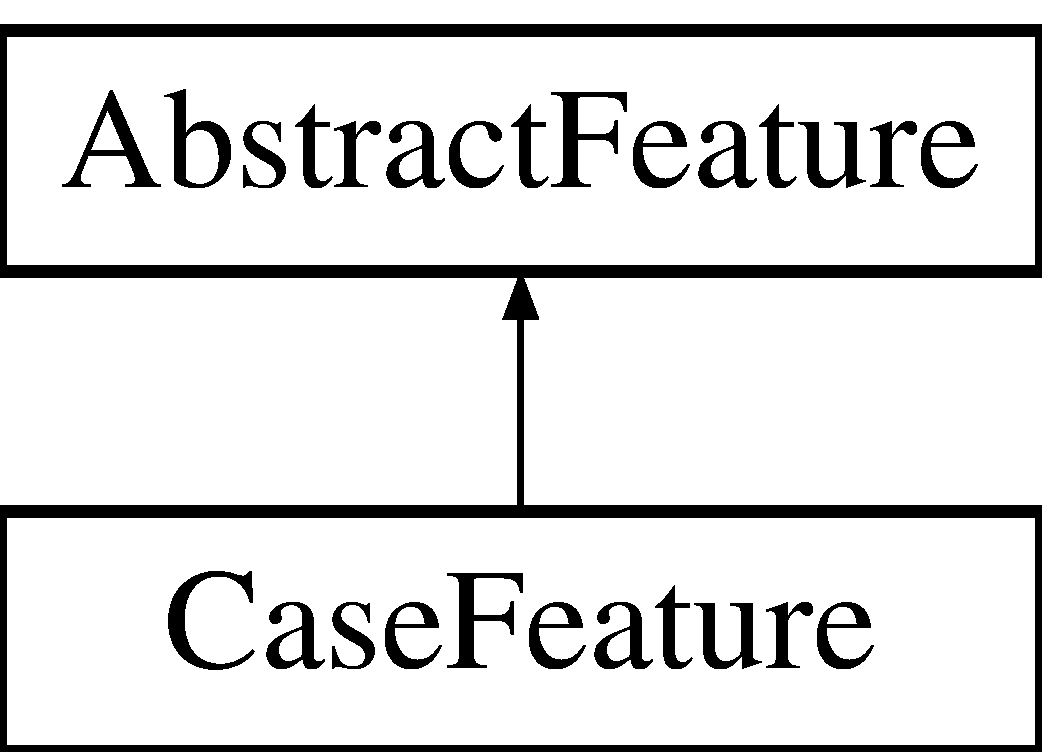
\includegraphics[height=2.000000cm]{class_abstract_feature}
\end{center}
\end{figure}
\subsection*{Public Member Functions}
\begin{DoxyCompactItemize}
\item 
\hyperlink{class_abstract_feature_acc855b1f84c6671d1fdb922a831ed170}{Abstract\+Feature} (int \hyperlink{class_abstract_feature_a3ac6f31b3e7a83ce4f73fab9f0139b7f}{id}, string \hyperlink{class_abstract_feature_a48465ede21b778021ea03b56d2117bc8}{name}, Type \hyperlink{class_abstract_feature_ac65cf0de277a8a62b6b1e1bdc249b237}{type})
\begin{DoxyCompactList}\small\item\em Construtor da classe \hyperlink{class_abstract_feature}{Abstract\+Feature}. \end{DoxyCompactList}\end{DoxyCompactItemize}
\subsection*{Public Attributes}
\begin{DoxyCompactItemize}
\item 
int \hyperlink{class_abstract_feature_a3ac6f31b3e7a83ce4f73fab9f0139b7f}{id}
\begin{DoxyCompactList}\small\item\em Identificador do atributo. \end{DoxyCompactList}\item 
string \hyperlink{class_abstract_feature_a48465ede21b778021ea03b56d2117bc8}{name}
\begin{DoxyCompactList}\small\item\em Nome do atributo. \end{DoxyCompactList}\item 
string \hyperlink{class_abstract_feature_ac65cf0de277a8a62b6b1e1bdc249b237}{type}
\begin{DoxyCompactList}\small\item\em Tipo de dado do atributo. \end{DoxyCompactList}\end{DoxyCompactItemize}


\subsection{Detailed Description}
Classe abstrata que representa a estrutura básica de um atributo. 



Definition at line 8 of file Abstract\+Feature.\+cs.



\subsection{Constructor \& Destructor Documentation}
\hypertarget{class_abstract_feature_acc855b1f84c6671d1fdb922a831ed170}{}\label{class_abstract_feature_acc855b1f84c6671d1fdb922a831ed170} 
\index{Abstract\+Feature@{Abstract\+Feature}!Abstract\+Feature@{Abstract\+Feature}}
\index{Abstract\+Feature@{Abstract\+Feature}!Abstract\+Feature@{Abstract\+Feature}}
\subsubsection{\texorpdfstring{Abstract\+Feature()}{AbstractFeature()}}
{\footnotesize\ttfamily Abstract\+Feature.\+Abstract\+Feature (\begin{DoxyParamCaption}\item[{int}]{id,  }\item[{string}]{name,  }\item[{Type}]{type }\end{DoxyParamCaption})}



Construtor da classe \hyperlink{class_abstract_feature}{Abstract\+Feature}. 


\begin{DoxyParams}{Parameters}
{\em id} & Identificador do novo atributo.\\
\hline
{\em name} & Nome do novo atributo.\\
\hline
{\em type} & Tipo de dado do novo atributo.\\
\hline
\end{DoxyParams}


Definition at line 31 of file Abstract\+Feature.\+cs.



\subsection{Member Data Documentation}
\hypertarget{class_abstract_feature_a3ac6f31b3e7a83ce4f73fab9f0139b7f}{}\label{class_abstract_feature_a3ac6f31b3e7a83ce4f73fab9f0139b7f} 
\index{Abstract\+Feature@{Abstract\+Feature}!id@{id}}
\index{id@{id}!Abstract\+Feature@{Abstract\+Feature}}
\subsubsection{\texorpdfstring{id}{id}}
{\footnotesize\ttfamily int Abstract\+Feature.\+id}



Identificador do atributo. 



Definition at line 13 of file Abstract\+Feature.\+cs.

\hypertarget{class_abstract_feature_a48465ede21b778021ea03b56d2117bc8}{}\label{class_abstract_feature_a48465ede21b778021ea03b56d2117bc8} 
\index{Abstract\+Feature@{Abstract\+Feature}!name@{name}}
\index{name@{name}!Abstract\+Feature@{Abstract\+Feature}}
\subsubsection{\texorpdfstring{name}{name}}
{\footnotesize\ttfamily string Abstract\+Feature.\+name}



Nome do atributo. 



Definition at line 18 of file Abstract\+Feature.\+cs.

\hypertarget{class_abstract_feature_ac65cf0de277a8a62b6b1e1bdc249b237}{}\label{class_abstract_feature_ac65cf0de277a8a62b6b1e1bdc249b237} 
\index{Abstract\+Feature@{Abstract\+Feature}!type@{type}}
\index{type@{type}!Abstract\+Feature@{Abstract\+Feature}}
\subsubsection{\texorpdfstring{type}{type}}
{\footnotesize\ttfamily string Abstract\+Feature.\+type}



Tipo de dado do atributo. 



Definition at line 23 of file Abstract\+Feature.\+cs.



The documentation for this class was generated from the following file\+:\begin{DoxyCompactItemize}
\item 
Abstract\+Classes/\hyperlink{_abstract_feature_8cs}{Abstract\+Feature.\+cs}\end{DoxyCompactItemize}

\hypertarget{class_abstract_global_similarity}{}\section{Abstract\+Global\+Similarity Class Reference}
\label{class_abstract_global_similarity}\index{Abstract\+Global\+Similarity@{Abstract\+Global\+Similarity}}


Classe abstrata que representa uma medida de similaridade global que será implementada na biblioteca C\+BR.  


Inheritance diagram for Abstract\+Global\+Similarity\+:\begin{figure}[H]
\begin{center}
\leavevmode
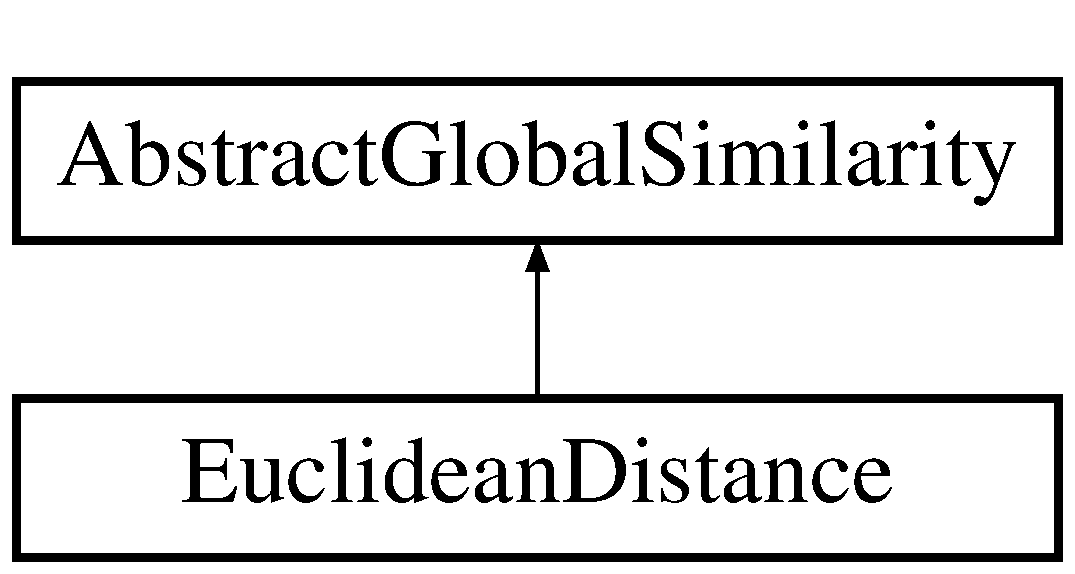
\includegraphics[height=2.000000cm]{class_abstract_global_similarity}
\end{center}
\end{figure}
\subsection*{Public Member Functions}
\begin{DoxyCompactItemize}
\item 
\hyperlink{class_abstract_global_similarity_ac13f827a8680ef4b6ee0d40911969f16}{Abstract\+Global\+Similarity} (\hyperlink{class_consult_structure}{Consult\+Structure} \hyperlink{class_abstract_global_similarity_a471ea41af416fd702d48f3b143416e66}{consult\+Structure})
\begin{DoxyCompactList}\small\item\em Construtor da classe \hyperlink{class_abstract_global_similarity}{Abstract\+Global\+Similarity}. \end{DoxyCompactList}\item 
abstract float \hyperlink{class_abstract_global_similarity_a4b97677ae2f5a0bdee41019b40b45114}{Get\+Similarity} (\hyperlink{class_case}{Case} search\+Case, \hyperlink{class_case}{Case} retrieve\+Case)
\begin{DoxyCompactList}\small\item\em Método abstrato que deve ser implementado por todas as classes que extenderem a classe \hyperlink{class_abstract_global_similarity}{Abstract\+Global\+Similarity}. \end{DoxyCompactList}\end{DoxyCompactItemize}
\subsection*{Public Attributes}
\begin{DoxyCompactItemize}
\item 
\hyperlink{class_consult_structure}{Consult\+Structure} \hyperlink{class_abstract_global_similarity_a471ea41af416fd702d48f3b143416e66}{consult\+Structure}
\begin{DoxyCompactList}\small\item\em Estrutura da consulta que será informada por cada classe que extender a classe \hyperlink{class_abstract_global_similarity}{Abstract\+Global\+Similarity}. \end{DoxyCompactList}\end{DoxyCompactItemize}


\subsection{Detailed Description}
Classe abstrata que representa uma medida de similaridade global que será implementada na biblioteca C\+BR. 



Definition at line 5 of file Abstract\+Global\+Similarity.\+cs.



\subsection{Constructor \& Destructor Documentation}
\hypertarget{class_abstract_global_similarity_ac13f827a8680ef4b6ee0d40911969f16}{}\label{class_abstract_global_similarity_ac13f827a8680ef4b6ee0d40911969f16} 
\index{Abstract\+Global\+Similarity@{Abstract\+Global\+Similarity}!Abstract\+Global\+Similarity@{Abstract\+Global\+Similarity}}
\index{Abstract\+Global\+Similarity@{Abstract\+Global\+Similarity}!Abstract\+Global\+Similarity@{Abstract\+Global\+Similarity}}
\subsubsection{\texorpdfstring{Abstract\+Global\+Similarity()}{AbstractGlobalSimilarity()}}
{\footnotesize\ttfamily Abstract\+Global\+Similarity.\+Abstract\+Global\+Similarity (\begin{DoxyParamCaption}\item[{\hyperlink{class_consult_structure}{Consult\+Structure}}]{consult\+Structure }\end{DoxyParamCaption})}



Construtor da classe \hyperlink{class_abstract_global_similarity}{Abstract\+Global\+Similarity}. 


\begin{DoxyParams}{Parameters}
{\em consult\+Structure} & Estrutura da consulta.\\
\hline
\end{DoxyParams}


Definition at line 16 of file Abstract\+Global\+Similarity.\+cs.



\subsection{Member Function Documentation}
\hypertarget{class_abstract_global_similarity_a4b97677ae2f5a0bdee41019b40b45114}{}\label{class_abstract_global_similarity_a4b97677ae2f5a0bdee41019b40b45114} 
\index{Abstract\+Global\+Similarity@{Abstract\+Global\+Similarity}!Get\+Similarity@{Get\+Similarity}}
\index{Get\+Similarity@{Get\+Similarity}!Abstract\+Global\+Similarity@{Abstract\+Global\+Similarity}}
\subsubsection{\texorpdfstring{Get\+Similarity()}{GetSimilarity()}}
{\footnotesize\ttfamily abstract float Abstract\+Global\+Similarity.\+Get\+Similarity (\begin{DoxyParamCaption}\item[{\hyperlink{class_case}{Case}}]{search\+Case,  }\item[{\hyperlink{class_case}{Case}}]{retrieve\+Case }\end{DoxyParamCaption})\hspace{0.3cm}{\ttfamily [pure virtual]}}



Método abstrato que deve ser implementado por todas as classes que extenderem a classe \hyperlink{class_abstract_global_similarity}{Abstract\+Global\+Similarity}. 


\begin{DoxyParams}{Parameters}
{\em search\+Case} & Caso utilizado como consulta.\\
\hline
{\em retrieve\+Case} & Caso recuperado da base de casos.\\
\hline
\end{DoxyParams}
\begin{DoxyReturn}{Returns}
Valor de similardade entre os casos c1 e c2.
\end{DoxyReturn}


Implemented in \hyperlink{class_euclidean_distance_a1b27b1fd06df3e3defca37187634951e}{Euclidean\+Distance}.



\subsection{Member Data Documentation}
\hypertarget{class_abstract_global_similarity_a471ea41af416fd702d48f3b143416e66}{}\label{class_abstract_global_similarity_a471ea41af416fd702d48f3b143416e66} 
\index{Abstract\+Global\+Similarity@{Abstract\+Global\+Similarity}!consult\+Structure@{consult\+Structure}}
\index{consult\+Structure@{consult\+Structure}!Abstract\+Global\+Similarity@{Abstract\+Global\+Similarity}}
\subsubsection{\texorpdfstring{consult\+Structure}{consultStructure}}
{\footnotesize\ttfamily \hyperlink{class_consult_structure}{Consult\+Structure} Abstract\+Global\+Similarity.\+consult\+Structure}



Estrutura da consulta que será informada por cada classe que extender a classe \hyperlink{class_abstract_global_similarity}{Abstract\+Global\+Similarity}. 



Definition at line 10 of file Abstract\+Global\+Similarity.\+cs.



The documentation for this class was generated from the following file\+:\begin{DoxyCompactItemize}
\item 
Abstract\+Classes/\hyperlink{_abstract_global_similarity_8cs}{Abstract\+Global\+Similarity.\+cs}\end{DoxyCompactItemize}

\hypertarget{class_abstract_local_similarity}{}\section{Abstract\+Local\+Similarity Class Reference}
\label{class_abstract_local_similarity}\index{Abstract\+Local\+Similarity@{Abstract\+Local\+Similarity}}


Classe abstrata que representa uma medida de similaridade local que será implementada na biblioteca C\+BR.  


Inheritance diagram for Abstract\+Local\+Similarity\+:\begin{figure}[H]
\begin{center}
\leavevmode
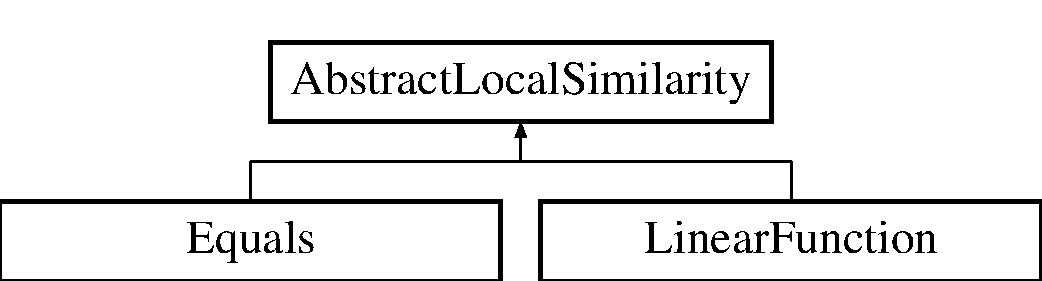
\includegraphics[height=2.000000cm]{class_abstract_local_similarity}
\end{center}
\end{figure}
\subsection*{Public Member Functions}
\begin{DoxyCompactItemize}
\item 
\hyperlink{class_abstract_local_similarity_a211b136bd5cd1525f3e4637868252696}{Abstract\+Local\+Similarity} ()
\begin{DoxyCompactList}\small\item\em Construtor da classe \hyperlink{class_abstract_local_similarity}{Abstract\+Local\+Similarity}. \end{DoxyCompactList}\item 
abstract float \hyperlink{class_abstract_local_similarity_a6c51b1fe09e99d509da0d3634225ca36}{Get\+Similarity} (\hyperlink{class_consult_params}{Consult\+Params} consult\+Params, \hyperlink{class_case}{Case} search\+Case, \hyperlink{class_case}{Case} retrieve\+Case)
\begin{DoxyCompactList}\small\item\em Método abstrato que deve ser implementado por todas as classes que extenderem a classe \hyperlink{class_abstract_local_similarity}{Abstract\+Local\+Similarity}. \end{DoxyCompactList}\end{DoxyCompactItemize}


\subsection{Detailed Description}
Classe abstrata que representa uma medida de similaridade local que será implementada na biblioteca C\+BR. 



Definition at line 6 of file Abstract\+Local\+Similarity.\+cs.



\subsection{Constructor \& Destructor Documentation}
\hypertarget{class_abstract_local_similarity_a211b136bd5cd1525f3e4637868252696}{}\label{class_abstract_local_similarity_a211b136bd5cd1525f3e4637868252696} 
\index{Abstract\+Local\+Similarity@{Abstract\+Local\+Similarity}!Abstract\+Local\+Similarity@{Abstract\+Local\+Similarity}}
\index{Abstract\+Local\+Similarity@{Abstract\+Local\+Similarity}!Abstract\+Local\+Similarity@{Abstract\+Local\+Similarity}}
\subsubsection{\texorpdfstring{Abstract\+Local\+Similarity()}{AbstractLocalSimilarity()}}
{\footnotesize\ttfamily Abstract\+Local\+Similarity.\+Abstract\+Local\+Similarity (\begin{DoxyParamCaption}{ }\end{DoxyParamCaption})}



Construtor da classe \hyperlink{class_abstract_local_similarity}{Abstract\+Local\+Similarity}. 



Definition at line 11 of file Abstract\+Local\+Similarity.\+cs.



\subsection{Member Function Documentation}
\hypertarget{class_abstract_local_similarity_a6c51b1fe09e99d509da0d3634225ca36}{}\label{class_abstract_local_similarity_a6c51b1fe09e99d509da0d3634225ca36} 
\index{Abstract\+Local\+Similarity@{Abstract\+Local\+Similarity}!Get\+Similarity@{Get\+Similarity}}
\index{Get\+Similarity@{Get\+Similarity}!Abstract\+Local\+Similarity@{Abstract\+Local\+Similarity}}
\subsubsection{\texorpdfstring{Get\+Similarity()}{GetSimilarity()}}
{\footnotesize\ttfamily abstract float Abstract\+Local\+Similarity.\+Get\+Similarity (\begin{DoxyParamCaption}\item[{\hyperlink{class_consult_params}{Consult\+Params}}]{consult\+Params,  }\item[{\hyperlink{class_case}{Case}}]{search\+Case,  }\item[{\hyperlink{class_case}{Case}}]{retrieve\+Case }\end{DoxyParamCaption})\hspace{0.3cm}{\ttfamily [pure virtual]}}



Método abstrato que deve ser implementado por todas as classes que extenderem a classe \hyperlink{class_abstract_local_similarity}{Abstract\+Local\+Similarity}. 


\begin{DoxyParams}{Parameters}
{\em consult\+Params} & Parâmetros da consulta.\\
\hline
{\em search\+Case} & Caso utilizado como consulta.\\
\hline
{\em retrieve\+Case} & Caso recuperado da base de casos.\\
\hline
\end{DoxyParams}
\begin{DoxyReturn}{Returns}

\end{DoxyReturn}


Implemented in \hyperlink{class_linear_function_addbfc2ff35037c40ae27c30e993e82ca}{Linear\+Function}, and \hyperlink{class_equals_a1b7c994cee3bf4ff55f6eaef5f31c871}{Equals}.



The documentation for this class was generated from the following file\+:\begin{DoxyCompactItemize}
\item 
Abstract\+Classes/\hyperlink{_abstract_local_similarity_8cs}{Abstract\+Local\+Similarity.\+cs}\end{DoxyCompactItemize}

\hypertarget{class_case}{}\section{Case Class Reference}
\label{class_case}\index{Case@{Case}}


Classe que representa um caso que compõem a base de casos. Composta por um identificador do caso e sua descrição do problema e solução.  


\subsection*{Public Member Functions}
\begin{DoxyCompactItemize}
\item 
\hyperlink{class_case_a78f4e108e49ef2fed453aa3e6cdd1ada}{Case} ()
\begin{DoxyCompactList}\small\item\em Construtor da classe \hyperlink{class_case}{Case}. \end{DoxyCompactList}\end{DoxyCompactItemize}
\subsection*{Public Attributes}
\begin{DoxyCompactItemize}
\item 
int \hyperlink{class_case_ac1ad667fc94d57692c17f5e3445096fc}{id}
\begin{DoxyCompactList}\small\item\em Identificador do caso. \end{DoxyCompactList}\item 
List$<$ \hyperlink{class_case_feature}{Case\+Feature} $>$ \hyperlink{class_case_a12be58e57891febe52b147a9266e54cb}{case\+Description}
\begin{DoxyCompactList}\small\item\em Descrição do problema a ser resolvido. \end{DoxyCompactList}\item 
List$<$ \hyperlink{class_case_feature}{Case\+Feature} $>$ \hyperlink{class_case_a0aa512e57a95843a20dd5190b043d793}{case\+Solution}
\begin{DoxyCompactList}\small\item\em Descrição da solução utilizada para resolver o problema. \end{DoxyCompactList}\end{DoxyCompactItemize}


\subsection{Detailed Description}
Classe que representa um caso que compõem a base de casos. Composta por um identificador do caso e sua descrição do problema e solução. 



Definition at line 8 of file Case.\+cs.



\subsection{Constructor \& Destructor Documentation}
\hypertarget{class_case_a78f4e108e49ef2fed453aa3e6cdd1ada}{}\label{class_case_a78f4e108e49ef2fed453aa3e6cdd1ada} 
\index{Case@{Case}!Case@{Case}}
\index{Case@{Case}!Case@{Case}}
\subsubsection{\texorpdfstring{Case()}{Case()}}
{\footnotesize\ttfamily Case.\+Case (\begin{DoxyParamCaption}{ }\end{DoxyParamCaption})}



Construtor da classe \hyperlink{class_case}{Case}. 



Definition at line 28 of file Case.\+cs.



\subsection{Member Data Documentation}
\hypertarget{class_case_a12be58e57891febe52b147a9266e54cb}{}\label{class_case_a12be58e57891febe52b147a9266e54cb} 
\index{Case@{Case}!case\+Description@{case\+Description}}
\index{case\+Description@{case\+Description}!Case@{Case}}
\subsubsection{\texorpdfstring{case\+Description}{caseDescription}}
{\footnotesize\ttfamily List$<$\hyperlink{class_case_feature}{Case\+Feature}$>$ Case.\+case\+Description}



Descrição do problema a ser resolvido. 



Definition at line 18 of file Case.\+cs.

\hypertarget{class_case_a0aa512e57a95843a20dd5190b043d793}{}\label{class_case_a0aa512e57a95843a20dd5190b043d793} 
\index{Case@{Case}!case\+Solution@{case\+Solution}}
\index{case\+Solution@{case\+Solution}!Case@{Case}}
\subsubsection{\texorpdfstring{case\+Solution}{caseSolution}}
{\footnotesize\ttfamily List$<$\hyperlink{class_case_feature}{Case\+Feature}$>$ Case.\+case\+Solution}



Descrição da solução utilizada para resolver o problema. 



Definition at line 23 of file Case.\+cs.

\hypertarget{class_case_ac1ad667fc94d57692c17f5e3445096fc}{}\label{class_case_ac1ad667fc94d57692c17f5e3445096fc} 
\index{Case@{Case}!id@{id}}
\index{id@{id}!Case@{Case}}
\subsubsection{\texorpdfstring{id}{id}}
{\footnotesize\ttfamily int Case.\+id}



Identificador do caso. 



Definition at line 13 of file Case.\+cs.



The documentation for this class was generated from the following file\+:\begin{DoxyCompactItemize}
\item 
Core/\hyperlink{_case_8cs}{Case.\+cs}\end{DoxyCompactItemize}

\hypertarget{class_case_base_connector}{}\section{Case\+Base\+Connector Class Reference}
\label{class_case_base_connector}\index{Case\+Base\+Connector@{Case\+Base\+Connector}}


Classe resposável por fazer a conexão entre a biblioteca C\+BR e a base de casos.  


\subsection*{Public Member Functions}
\begin{DoxyCompactItemize}
\item 
\hyperlink{class_case_base_connector_adb41d690fb4a06168c15b3b750c0cda2}{Case\+Base\+Connector} (string file\+Name)
\begin{DoxyCompactList}\small\item\em Construtor da classe \hyperlink{class_case_base_connector}{Case\+Base\+Connector}. \end{DoxyCompactList}\item 
void \hyperlink{class_case_base_connector_a6b5e35626b1b6a718bbdba83f153834b}{Load\+Case\+Base} ()
\begin{DoxyCompactList}\small\item\em Método que carrega todos os casos da base de casos na memória R\+AM. \end{DoxyCompactList}\item 
void \hyperlink{class_case_base_connector_a1aa00f0a3bcf25bafa6bab87ec1e455e}{Create\+Case\+Base} ()
\begin{DoxyCompactList}\small\item\em Método que cria a base de casos. \end{DoxyCompactList}\item 
\hyperlink{class_case}{Case} \hyperlink{class_case_base_connector_abca3ec961411fce4948f4ea5b40e9fb6}{Load\+Case} (int case\+Id)
\begin{DoxyCompactList}\small\item\em Método que carrega um caso da base de casos. \end{DoxyCompactList}\item 
void \hyperlink{class_case_base_connector_abfb6f1dae5b06827667d5f033736f7a0}{Add\+Case} (\hyperlink{class_case}{Case} new\+Case)
\begin{DoxyCompactList}\small\item\em Método que adiciona um novo caso na base de casos. \end{DoxyCompactList}\item 
void \hyperlink{class_case_base_connector_a1a85907a149e2bb4e3c198936e6f59d3}{Remove\+Case} (int case\+Id)
\begin{DoxyCompactList}\small\item\em Método que remove um caso da base de casos. \end{DoxyCompactList}\item 
void \hyperlink{class_case_base_connector_afc9618b6b8f22f9184e59a86086be239}{Edit\+Case} (int case\+Id, \hyperlink{class_case}{Case} new\+Case)
\begin{DoxyCompactList}\small\item\em Método que substitui um caso da base de casos por um novo caso. \end{DoxyCompactList}\end{DoxyCompactItemize}
\subsection*{Public Attributes}
\begin{DoxyCompactItemize}
\item 
List$<$ \hyperlink{class_case}{Case} $>$ \hyperlink{class_case_base_connector_afbbc563b42797bf19f8790f40e34425a}{case\+Base}
\begin{DoxyCompactList}\small\item\em Lista de casos presentes na base de casos. \end{DoxyCompactList}\end{DoxyCompactItemize}


\subsection{Detailed Description}
Classe resposável por fazer a conexão entre a biblioteca C\+BR e a base de casos. 



Definition at line 10 of file Case\+Base\+Connector.\+cs.



\subsection{Constructor \& Destructor Documentation}
\hypertarget{class_case_base_connector_adb41d690fb4a06168c15b3b750c0cda2}{}\label{class_case_base_connector_adb41d690fb4a06168c15b3b750c0cda2} 
\index{Case\+Base\+Connector@{Case\+Base\+Connector}!Case\+Base\+Connector@{Case\+Base\+Connector}}
\index{Case\+Base\+Connector@{Case\+Base\+Connector}!Case\+Base\+Connector@{Case\+Base\+Connector}}
\subsubsection{\texorpdfstring{Case\+Base\+Connector()}{CaseBaseConnector()}}
{\footnotesize\ttfamily Case\+Base\+Connector.\+Case\+Base\+Connector (\begin{DoxyParamCaption}\item[{string}]{file\+Name }\end{DoxyParamCaption})}



Construtor da classe \hyperlink{class_case_base_connector}{Case\+Base\+Connector}. 


\begin{DoxyParams}{Parameters}
{\em file\+Name} & Nome do arquivo que representa a base de casos.\\
\hline
\end{DoxyParams}


Definition at line 31 of file Case\+Base\+Connector.\+cs.



\subsection{Member Function Documentation}
\hypertarget{class_case_base_connector_abfb6f1dae5b06827667d5f033736f7a0}{}\label{class_case_base_connector_abfb6f1dae5b06827667d5f033736f7a0} 
\index{Case\+Base\+Connector@{Case\+Base\+Connector}!Add\+Case@{Add\+Case}}
\index{Add\+Case@{Add\+Case}!Case\+Base\+Connector@{Case\+Base\+Connector}}
\subsubsection{\texorpdfstring{Add\+Case()}{AddCase()}}
{\footnotesize\ttfamily void Case\+Base\+Connector.\+Add\+Case (\begin{DoxyParamCaption}\item[{\hyperlink{class_case}{Case}}]{new\+Case }\end{DoxyParamCaption})}



Método que adiciona um novo caso na base de casos. 


\begin{DoxyParams}{Parameters}
{\em new\+Case} & Novo caso a ser adicionado na base de casos.\\
\hline
\end{DoxyParams}


Definition at line 95 of file Case\+Base\+Connector.\+cs.

\hypertarget{class_case_base_connector_a1aa00f0a3bcf25bafa6bab87ec1e455e}{}\label{class_case_base_connector_a1aa00f0a3bcf25bafa6bab87ec1e455e} 
\index{Case\+Base\+Connector@{Case\+Base\+Connector}!Create\+Case\+Base@{Create\+Case\+Base}}
\index{Create\+Case\+Base@{Create\+Case\+Base}!Case\+Base\+Connector@{Case\+Base\+Connector}}
\subsubsection{\texorpdfstring{Create\+Case\+Base()}{CreateCaseBase()}}
{\footnotesize\ttfamily void Case\+Base\+Connector.\+Create\+Case\+Base (\begin{DoxyParamCaption}{ }\end{DoxyParamCaption})}



Método que cria a base de casos. 



Definition at line 56 of file Case\+Base\+Connector.\+cs.

\hypertarget{class_case_base_connector_afc9618b6b8f22f9184e59a86086be239}{}\label{class_case_base_connector_afc9618b6b8f22f9184e59a86086be239} 
\index{Case\+Base\+Connector@{Case\+Base\+Connector}!Edit\+Case@{Edit\+Case}}
\index{Edit\+Case@{Edit\+Case}!Case\+Base\+Connector@{Case\+Base\+Connector}}
\subsubsection{\texorpdfstring{Edit\+Case()}{EditCase()}}
{\footnotesize\ttfamily void Case\+Base\+Connector.\+Edit\+Case (\begin{DoxyParamCaption}\item[{int}]{case\+Id,  }\item[{\hyperlink{class_case}{Case}}]{new\+Case }\end{DoxyParamCaption})}



Método que substitui um caso da base de casos por um novo caso. 


\begin{DoxyParams}{Parameters}
{\em case\+Id} & Identificador do caso a ser alterado na base de casos.\\
\hline
{\em new\+Case} & Novo caso que alterará um caso presente na base de casos.\\
\hline
\end{DoxyParams}


Definition at line 123 of file Case\+Base\+Connector.\+cs.

\hypertarget{class_case_base_connector_abca3ec961411fce4948f4ea5b40e9fb6}{}\label{class_case_base_connector_abca3ec961411fce4948f4ea5b40e9fb6} 
\index{Case\+Base\+Connector@{Case\+Base\+Connector}!Load\+Case@{Load\+Case}}
\index{Load\+Case@{Load\+Case}!Case\+Base\+Connector@{Case\+Base\+Connector}}
\subsubsection{\texorpdfstring{Load\+Case()}{LoadCase()}}
{\footnotesize\ttfamily \hyperlink{class_case}{Case} Case\+Base\+Connector.\+Load\+Case (\begin{DoxyParamCaption}\item[{int}]{case\+Id }\end{DoxyParamCaption})}



Método que carrega um caso da base de casos. 


\begin{DoxyParams}{Parameters}
{\em case\+Id} & Identificador do caso a ser carregado.\\
\hline
\end{DoxyParams}
\begin{DoxyReturn}{Returns}

\end{DoxyReturn}


Definition at line 77 of file Case\+Base\+Connector.\+cs.

\hypertarget{class_case_base_connector_a6b5e35626b1b6a718bbdba83f153834b}{}\label{class_case_base_connector_a6b5e35626b1b6a718bbdba83f153834b} 
\index{Case\+Base\+Connector@{Case\+Base\+Connector}!Load\+Case\+Base@{Load\+Case\+Base}}
\index{Load\+Case\+Base@{Load\+Case\+Base}!Case\+Base\+Connector@{Case\+Base\+Connector}}
\subsubsection{\texorpdfstring{Load\+Case\+Base()}{LoadCaseBase()}}
{\footnotesize\ttfamily void Case\+Base\+Connector.\+Load\+Case\+Base (\begin{DoxyParamCaption}{ }\end{DoxyParamCaption})}



Método que carrega todos os casos da base de casos na memória R\+AM. 



Definition at line 40 of file Case\+Base\+Connector.\+cs.

\hypertarget{class_case_base_connector_a1a85907a149e2bb4e3c198936e6f59d3}{}\label{class_case_base_connector_a1a85907a149e2bb4e3c198936e6f59d3} 
\index{Case\+Base\+Connector@{Case\+Base\+Connector}!Remove\+Case@{Remove\+Case}}
\index{Remove\+Case@{Remove\+Case}!Case\+Base\+Connector@{Case\+Base\+Connector}}
\subsubsection{\texorpdfstring{Remove\+Case()}{RemoveCase()}}
{\footnotesize\ttfamily void Case\+Base\+Connector.\+Remove\+Case (\begin{DoxyParamCaption}\item[{int}]{case\+Id }\end{DoxyParamCaption})}



Método que remove um caso da base de casos. 


\begin{DoxyParams}{Parameters}
{\em case\+Id} & Identificador do caso a ser removido da base de casos.\\
\hline
\end{DoxyParams}


Definition at line 105 of file Case\+Base\+Connector.\+cs.



\subsection{Member Data Documentation}
\hypertarget{class_case_base_connector_afbbc563b42797bf19f8790f40e34425a}{}\label{class_case_base_connector_afbbc563b42797bf19f8790f40e34425a} 
\index{Case\+Base\+Connector@{Case\+Base\+Connector}!case\+Base@{case\+Base}}
\index{case\+Base@{case\+Base}!Case\+Base\+Connector@{Case\+Base\+Connector}}
\subsubsection{\texorpdfstring{case\+Base}{caseBase}}
{\footnotesize\ttfamily List$<$\hyperlink{class_case}{Case}$>$ Case\+Base\+Connector.\+case\+Base}



Lista de casos presentes na base de casos. 



Definition at line 15 of file Case\+Base\+Connector.\+cs.



The documentation for this class was generated from the following file\+:\begin{DoxyCompactItemize}
\item 
Core/\hyperlink{_case_base_connector_8cs}{Case\+Base\+Connector.\+cs}\end{DoxyCompactItemize}

\hypertarget{class_case_feature}{}\section{Case\+Feature Class Reference}
\label{class_case_feature}\index{Case\+Feature@{Case\+Feature}}


Classe que representa um atributo presente na descrição do problema ou solução de um caso.  


Inheritance diagram for Case\+Feature\+:\begin{figure}[H]
\begin{center}
\leavevmode
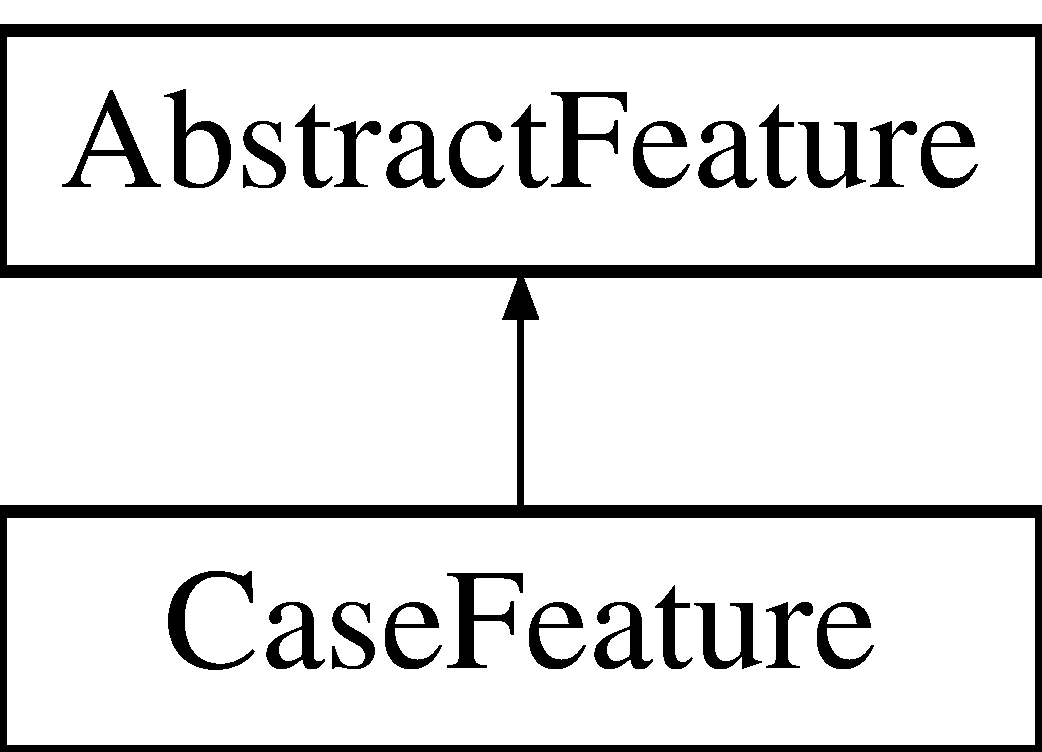
\includegraphics[height=2.000000cm]{class_case_feature}
\end{center}
\end{figure}
\subsection*{Public Member Functions}
\begin{DoxyCompactItemize}
\item 
\hyperlink{class_case_feature_a9443dc93f40c63cc812c4102f15498c5}{Case\+Feature} (int \hyperlink{class_abstract_feature_a3ac6f31b3e7a83ce4f73fab9f0139b7f}{id}, string \hyperlink{class_abstract_feature_a48465ede21b778021ea03b56d2117bc8}{name}, Type \hyperlink{class_abstract_feature_ac65cf0de277a8a62b6b1e1bdc249b237}{type}, object \hyperlink{class_case_feature_a1aa9c93657c27e6a8debdf71a40f5b89}{value})
\begin{DoxyCompactList}\small\item\em Construtor da classe \hyperlink{class_case_feature}{Case\+Feature}. \end{DoxyCompactList}\item 
\hyperlink{class_case_feature_afcbe5b640972620a71192f3b45c8cbcc}{Case\+Feature} (int \hyperlink{class_abstract_feature_a3ac6f31b3e7a83ce4f73fab9f0139b7f}{id}, string \hyperlink{class_abstract_feature_a48465ede21b778021ea03b56d2117bc8}{name}, Type \hyperlink{class_abstract_feature_ac65cf0de277a8a62b6b1e1bdc249b237}{type})
\begin{DoxyCompactList}\small\item\em Construtor da classe \hyperlink{class_case_feature}{Case\+Feature}. \end{DoxyCompactList}\end{DoxyCompactItemize}
\subsection*{Public Attributes}
\begin{DoxyCompactItemize}
\item 
string \hyperlink{class_case_feature_a1aa9c93657c27e6a8debdf71a40f5b89}{value}
\begin{DoxyCompactList}\small\item\em Valor do atributo. \end{DoxyCompactList}\end{DoxyCompactItemize}


\subsection{Detailed Description}
Classe que representa um atributo presente na descrição do problema ou solução de um caso. 



Definition at line 7 of file Case\+Feature.\+cs.



\subsection{Constructor \& Destructor Documentation}
\hypertarget{class_case_feature_a9443dc93f40c63cc812c4102f15498c5}{}\label{class_case_feature_a9443dc93f40c63cc812c4102f15498c5} 
\index{Case\+Feature@{Case\+Feature}!Case\+Feature@{Case\+Feature}}
\index{Case\+Feature@{Case\+Feature}!Case\+Feature@{Case\+Feature}}
\subsubsection{\texorpdfstring{Case\+Feature()}{CaseFeature()}\hspace{0.1cm}{\footnotesize\ttfamily [1/2]}}
{\footnotesize\ttfamily Case\+Feature.\+Case\+Feature (\begin{DoxyParamCaption}\item[{int}]{id,  }\item[{string}]{name,  }\item[{Type}]{type,  }\item[{object}]{value }\end{DoxyParamCaption})}



Construtor da classe \hyperlink{class_case_feature}{Case\+Feature}. 


\begin{DoxyParams}{Parameters}
{\em id} & Identificador do atributo.\\
\hline
{\em name} & Nome do atributo.\\
\hline
{\em type} & Tipo de dado do atributo.\\
\hline
{\em value} & Valor do atributo.\\
\hline
\end{DoxyParams}


Definition at line 21 of file Case\+Feature.\+cs.

\hypertarget{class_case_feature_afcbe5b640972620a71192f3b45c8cbcc}{}\label{class_case_feature_afcbe5b640972620a71192f3b45c8cbcc} 
\index{Case\+Feature@{Case\+Feature}!Case\+Feature@{Case\+Feature}}
\index{Case\+Feature@{Case\+Feature}!Case\+Feature@{Case\+Feature}}
\subsubsection{\texorpdfstring{Case\+Feature()}{CaseFeature()}\hspace{0.1cm}{\footnotesize\ttfamily [2/2]}}
{\footnotesize\ttfamily Case\+Feature.\+Case\+Feature (\begin{DoxyParamCaption}\item[{int}]{id,  }\item[{string}]{name,  }\item[{Type}]{type }\end{DoxyParamCaption})}



Construtor da classe \hyperlink{class_case_feature}{Case\+Feature}. 


\begin{DoxyParams}{Parameters}
{\em id} & Identificador do atributo.\\
\hline
{\em name} & Nome do atributo.\\
\hline
{\em type} & Tipo de dado do atributo.\\
\hline
\end{DoxyParams}


Definition at line 32 of file Case\+Feature.\+cs.



\subsection{Member Data Documentation}
\hypertarget{class_case_feature_a1aa9c93657c27e6a8debdf71a40f5b89}{}\label{class_case_feature_a1aa9c93657c27e6a8debdf71a40f5b89} 
\index{Case\+Feature@{Case\+Feature}!value@{value}}
\index{value@{value}!Case\+Feature@{Case\+Feature}}
\subsubsection{\texorpdfstring{value}{value}}
{\footnotesize\ttfamily string Case\+Feature.\+value}



Valor do atributo. 



Definition at line 12 of file Case\+Feature.\+cs.



The documentation for this class was generated from the following file\+:\begin{DoxyCompactItemize}
\item 
Core/\hyperlink{_case_feature_8cs}{Case\+Feature.\+cs}\end{DoxyCompactItemize}

\hypertarget{class_c_b_r_a_p_i}{}\section{C\+B\+R\+A\+PI Class Reference}
\label{class_c_b_r_a_p_i}\index{C\+B\+R\+A\+PI@{C\+B\+R\+A\+PI}}


Classe que deve ser instanciada para ser possível utilizar a biblioteca C\+BR.  


\subsection*{Public Member Functions}
\begin{DoxyCompactItemize}
\item 
\hyperlink{class_c_b_r_a_p_i_a6e4d8b523865ebbc550a50ff1785231b}{C\+B\+R\+A\+PI} ()
\begin{DoxyCompactList}\small\item\em Construtor da classe \hyperlink{class_c_b_r_a_p_i}{C\+B\+R\+A\+PI}. \end{DoxyCompactList}\item 
\hyperlink{class_c_b_r_a_p_i_a9e521eefe067de857bcc86990d64256e}{C\+B\+R\+A\+PI} (string file\+Name)
\begin{DoxyCompactList}\small\item\em Construtor da classe \hyperlink{class_c_b_r_a_p_i}{C\+B\+R\+A\+PI}. \end{DoxyCompactList}\item 
void \hyperlink{class_c_b_r_a_p_i_a887ddacca4fd9f79d20f8b392b3e8a8e}{Add\+Case} (\hyperlink{class_case}{Case} new\+Case)
\begin{DoxyCompactList}\small\item\em Método que passa um novo caso para a classe \hyperlink{class_case_base_connector}{Case\+Base\+Connector} adicionar na base de casos. \end{DoxyCompactList}\item 
void \hyperlink{class_c_b_r_a_p_i_a592d54dfb86d74154ed0e74dc3aa6f73}{Remove\+Case} (int case\+ID)
\begin{DoxyCompactList}\small\item\em Método que informa a classe \hyperlink{class_case_base_connector}{Case\+Base\+Connector} qual caso deve ser removido. \end{DoxyCompactList}\item 
void \hyperlink{class_c_b_r_a_p_i_a80d48f14d29ee6c2ac4bacff19ea9c0c}{Edit\+Case} (int case\+ID, \hyperlink{class_case}{Case} new\+Case)
\begin{DoxyCompactList}\small\item\em Método que informa a classe \hyperlink{class_case_base_connector}{Case\+Base\+Connector} qual caso deve ser editado. \end{DoxyCompactList}\item 
List$<$ \hyperlink{class_result}{Result} $>$ \hyperlink{class_c_b_r_a_p_i_af1992aae5101968f2a851f1ac1c044d7}{Retrieve} (\hyperlink{class_case}{Case} search\+Case, \hyperlink{class_consult_structure}{Consult\+Structure} consult\+Structure)
\begin{DoxyCompactList}\small\item\em Realiza e etapa de recuperação do ciclo de C\+BR. \end{DoxyCompactList}\end{DoxyCompactItemize}


\subsection{Detailed Description}
Classe que deve ser instanciada para ser possível utilizar a biblioteca C\+BR. 



Definition at line 6 of file C\+B\+R\+A\+P\+I.\+cs.



\subsection{Constructor \& Destructor Documentation}
\hypertarget{class_c_b_r_a_p_i_a6e4d8b523865ebbc550a50ff1785231b}{}\label{class_c_b_r_a_p_i_a6e4d8b523865ebbc550a50ff1785231b} 
\index{C\+B\+R\+A\+PI@{C\+B\+R\+A\+PI}!C\+B\+R\+A\+PI@{C\+B\+R\+A\+PI}}
\index{C\+B\+R\+A\+PI@{C\+B\+R\+A\+PI}!C\+B\+R\+A\+PI@{C\+B\+R\+A\+PI}}
\subsubsection{\texorpdfstring{C\+B\+R\+A\+P\+I()}{CBRAPI()}\hspace{0.1cm}{\footnotesize\ttfamily [1/2]}}
{\footnotesize\ttfamily C\+B\+R\+A\+P\+I.\+C\+B\+R\+A\+PI (\begin{DoxyParamCaption}{ }\end{DoxyParamCaption})}



Construtor da classe \hyperlink{class_c_b_r_a_p_i}{C\+B\+R\+A\+PI}. 



Definition at line 17 of file C\+B\+R\+A\+P\+I.\+cs.

\hypertarget{class_c_b_r_a_p_i_a9e521eefe067de857bcc86990d64256e}{}\label{class_c_b_r_a_p_i_a9e521eefe067de857bcc86990d64256e} 
\index{C\+B\+R\+A\+PI@{C\+B\+R\+A\+PI}!C\+B\+R\+A\+PI@{C\+B\+R\+A\+PI}}
\index{C\+B\+R\+A\+PI@{C\+B\+R\+A\+PI}!C\+B\+R\+A\+PI@{C\+B\+R\+A\+PI}}
\subsubsection{\texorpdfstring{C\+B\+R\+A\+P\+I()}{CBRAPI()}\hspace{0.1cm}{\footnotesize\ttfamily [2/2]}}
{\footnotesize\ttfamily C\+B\+R\+A\+P\+I.\+C\+B\+R\+A\+PI (\begin{DoxyParamCaption}\item[{string}]{file\+Name }\end{DoxyParamCaption})}



Construtor da classe \hyperlink{class_c_b_r_a_p_i}{C\+B\+R\+A\+PI}. 


\begin{DoxyParams}{Parameters}
{\em file\+Name} & Nome do arquivo que represeta a base de casos.\\
\hline
\end{DoxyParams}


Definition at line 28 of file C\+B\+R\+A\+P\+I.\+cs.



\subsection{Member Function Documentation}
\hypertarget{class_c_b_r_a_p_i_a887ddacca4fd9f79d20f8b392b3e8a8e}{}\label{class_c_b_r_a_p_i_a887ddacca4fd9f79d20f8b392b3e8a8e} 
\index{C\+B\+R\+A\+PI@{C\+B\+R\+A\+PI}!Add\+Case@{Add\+Case}}
\index{Add\+Case@{Add\+Case}!C\+B\+R\+A\+PI@{C\+B\+R\+A\+PI}}
\subsubsection{\texorpdfstring{Add\+Case()}{AddCase()}}
{\footnotesize\ttfamily void C\+B\+R\+A\+P\+I.\+Add\+Case (\begin{DoxyParamCaption}\item[{\hyperlink{class_case}{Case}}]{new\+Case }\end{DoxyParamCaption})}



Método que passa um novo caso para a classe \hyperlink{class_case_base_connector}{Case\+Base\+Connector} adicionar na base de casos. 


\begin{DoxyParams}{Parameters}
{\em new\+Case} & Novo caso.\\
\hline
\end{DoxyParams}


Definition at line 39 of file C\+B\+R\+A\+P\+I.\+cs.

\hypertarget{class_c_b_r_a_p_i_a80d48f14d29ee6c2ac4bacff19ea9c0c}{}\label{class_c_b_r_a_p_i_a80d48f14d29ee6c2ac4bacff19ea9c0c} 
\index{C\+B\+R\+A\+PI@{C\+B\+R\+A\+PI}!Edit\+Case@{Edit\+Case}}
\index{Edit\+Case@{Edit\+Case}!C\+B\+R\+A\+PI@{C\+B\+R\+A\+PI}}
\subsubsection{\texorpdfstring{Edit\+Case()}{EditCase()}}
{\footnotesize\ttfamily void C\+B\+R\+A\+P\+I.\+Edit\+Case (\begin{DoxyParamCaption}\item[{int}]{case\+ID,  }\item[{\hyperlink{class_case}{Case}}]{new\+Case }\end{DoxyParamCaption})}



Método que informa a classe \hyperlink{class_case_base_connector}{Case\+Base\+Connector} qual caso deve ser editado. 


\begin{DoxyParams}{Parameters}
{\em case\+ID} & Identificador do caso e ser editado.\\
\hline
{\em new\+Case} & Novo caso que irá substituir um já existente.\\
\hline
\end{DoxyParams}


Definition at line 58 of file C\+B\+R\+A\+P\+I.\+cs.

\hypertarget{class_c_b_r_a_p_i_a592d54dfb86d74154ed0e74dc3aa6f73}{}\label{class_c_b_r_a_p_i_a592d54dfb86d74154ed0e74dc3aa6f73} 
\index{C\+B\+R\+A\+PI@{C\+B\+R\+A\+PI}!Remove\+Case@{Remove\+Case}}
\index{Remove\+Case@{Remove\+Case}!C\+B\+R\+A\+PI@{C\+B\+R\+A\+PI}}
\subsubsection{\texorpdfstring{Remove\+Case()}{RemoveCase()}}
{\footnotesize\ttfamily void C\+B\+R\+A\+P\+I.\+Remove\+Case (\begin{DoxyParamCaption}\item[{int}]{case\+ID }\end{DoxyParamCaption})}



Método que informa a classe \hyperlink{class_case_base_connector}{Case\+Base\+Connector} qual caso deve ser removido. 


\begin{DoxyParams}{Parameters}
{\em case\+ID} & Identificador do caso a ser removido.\\
\hline
\end{DoxyParams}


Definition at line 48 of file C\+B\+R\+A\+P\+I.\+cs.

\hypertarget{class_c_b_r_a_p_i_af1992aae5101968f2a851f1ac1c044d7}{}\label{class_c_b_r_a_p_i_af1992aae5101968f2a851f1ac1c044d7} 
\index{C\+B\+R\+A\+PI@{C\+B\+R\+A\+PI}!Retrieve@{Retrieve}}
\index{Retrieve@{Retrieve}!C\+B\+R\+A\+PI@{C\+B\+R\+A\+PI}}
\subsubsection{\texorpdfstring{Retrieve()}{Retrieve()}}
{\footnotesize\ttfamily List$<$\hyperlink{class_result}{Result}$>$ C\+B\+R\+A\+P\+I.\+Retrieve (\begin{DoxyParamCaption}\item[{\hyperlink{class_case}{Case}}]{search\+Case,  }\item[{\hyperlink{class_consult_structure}{Consult\+Structure}}]{consult\+Structure }\end{DoxyParamCaption})}



Realiza e etapa de recuperação do ciclo de C\+BR. 


\begin{DoxyParams}{Parameters}
{\em search\+Case} & Caso de consulta.\\
\hline
\end{DoxyParams}
\begin{DoxyReturn}{Returns}

\end{DoxyReturn}


Definition at line 68 of file C\+B\+R\+A\+P\+I.\+cs.



The documentation for this class was generated from the following file\+:\begin{DoxyCompactItemize}
\item 
Core/\hyperlink{_c_b_r_a_p_i_8cs}{C\+B\+R\+A\+P\+I.\+cs}\end{DoxyCompactItemize}

\hypertarget{class_consult_params}{}\section{Consult\+Params Class Reference}
\label{class_consult_params}\index{Consult\+Params@{Consult\+Params}}


Classe que contém os parâmetros da consulta que serão utilizados para a análise de similaridade entre dois casos.  


\subsection*{Public Member Functions}
\begin{DoxyCompactItemize}
\item 
\hyperlink{class_consult_params_a08afdf573f25bd9af48bde1f43310389}{Consult\+Params} (List$<$ int $>$ \hyperlink{class_consult_params_a48d859e63fc26ee92c05696e73180b9f}{indexes}, float \hyperlink{class_consult_params_aedab07a8d28bff47cbc569778533493e}{weight}, \hyperlink{class_abstract_local_similarity}{Abstract\+Local\+Similarity} \hyperlink{class_consult_params_a1910c45b23c7c0654518ba528d3e5a69}{local\+Similarity})
\begin{DoxyCompactList}\small\item\em Construtor da classe \hyperlink{class_consult_params}{Consult\+Params}. \end{DoxyCompactList}\end{DoxyCompactItemize}
\subsection*{Public Attributes}
\begin{DoxyCompactItemize}
\item 
float \hyperlink{class_consult_params_aedab07a8d28bff47cbc569778533493e}{weight}
\begin{DoxyCompactList}\small\item\em Peso da consulta na análise de similaridade. \end{DoxyCompactList}\item 
\hyperlink{class_abstract_local_similarity}{Abstract\+Local\+Similarity} \hyperlink{class_consult_params_a1910c45b23c7c0654518ba528d3e5a69}{local\+Similarity}
\begin{DoxyCompactList}\small\item\em Função de similaridade local que será utilizada na consulta. \end{DoxyCompactList}\item 
List$<$ int $>$ \hyperlink{class_consult_params_a48d859e63fc26ee92c05696e73180b9f}{indexes}
\begin{DoxyCompactList}\small\item\em Índice dos atributos utilizados na consulta. \end{DoxyCompactList}\end{DoxyCompactItemize}


\subsection{Detailed Description}
Classe que contém os parâmetros da consulta que serão utilizados para a análise de similaridade entre dois casos. 



Definition at line 8 of file Consult\+Params.\+cs.



\subsection{Constructor \& Destructor Documentation}
\hypertarget{class_consult_params_a08afdf573f25bd9af48bde1f43310389}{}\label{class_consult_params_a08afdf573f25bd9af48bde1f43310389} 
\index{Consult\+Params@{Consult\+Params}!Consult\+Params@{Consult\+Params}}
\index{Consult\+Params@{Consult\+Params}!Consult\+Params@{Consult\+Params}}
\subsubsection{\texorpdfstring{Consult\+Params()}{ConsultParams()}}
{\footnotesize\ttfamily Consult\+Params.\+Consult\+Params (\begin{DoxyParamCaption}\item[{List$<$ int $>$}]{indexes,  }\item[{float}]{weight,  }\item[{\hyperlink{class_abstract_local_similarity}{Abstract\+Local\+Similarity}}]{local\+Similarity }\end{DoxyParamCaption})}



Construtor da classe \hyperlink{class_consult_params}{Consult\+Params}. 


\begin{DoxyParams}{Parameters}
{\em indexes} & Índice dos atributos utilizados na consulta.\\
\hline
{\em weight} & Peso da consulta na análise de similaridade.\\
\hline
{\em local\+Similarity} & Função de similaridade local que será utilizada na consulta.\\
\hline
\end{DoxyParams}


Definition at line 31 of file Consult\+Params.\+cs.



\subsection{Member Data Documentation}
\hypertarget{class_consult_params_a48d859e63fc26ee92c05696e73180b9f}{}\label{class_consult_params_a48d859e63fc26ee92c05696e73180b9f} 
\index{Consult\+Params@{Consult\+Params}!indexes@{indexes}}
\index{indexes@{indexes}!Consult\+Params@{Consult\+Params}}
\subsubsection{\texorpdfstring{indexes}{indexes}}
{\footnotesize\ttfamily List$<$int$>$ Consult\+Params.\+indexes}



Índice dos atributos utilizados na consulta. 



Definition at line 23 of file Consult\+Params.\+cs.

\hypertarget{class_consult_params_a1910c45b23c7c0654518ba528d3e5a69}{}\label{class_consult_params_a1910c45b23c7c0654518ba528d3e5a69} 
\index{Consult\+Params@{Consult\+Params}!local\+Similarity@{local\+Similarity}}
\index{local\+Similarity@{local\+Similarity}!Consult\+Params@{Consult\+Params}}
\subsubsection{\texorpdfstring{local\+Similarity}{localSimilarity}}
{\footnotesize\ttfamily \hyperlink{class_abstract_local_similarity}{Abstract\+Local\+Similarity} Consult\+Params.\+local\+Similarity}



Função de similaridade local que será utilizada na consulta. 



Definition at line 18 of file Consult\+Params.\+cs.

\hypertarget{class_consult_params_aedab07a8d28bff47cbc569778533493e}{}\label{class_consult_params_aedab07a8d28bff47cbc569778533493e} 
\index{Consult\+Params@{Consult\+Params}!weight@{weight}}
\index{weight@{weight}!Consult\+Params@{Consult\+Params}}
\subsubsection{\texorpdfstring{weight}{weight}}
{\footnotesize\ttfamily float Consult\+Params.\+weight}



Peso da consulta na análise de similaridade. 



Definition at line 13 of file Consult\+Params.\+cs.



The documentation for this class was generated from the following file\+:\begin{DoxyCompactItemize}
\item 
Core/\hyperlink{_consult_params_8cs}{Consult\+Params.\+cs}\end{DoxyCompactItemize}

\hypertarget{class_consult_structure}{}\section{Consult\+Structure Class Reference}
\label{class_consult_structure}\index{Consult\+Structure@{Consult\+Structure}}


Classe que contém a estrutura de consulta que será utilizada na análise de similaridade entre os casos.  


\subsection*{Public Member Functions}
\begin{DoxyCompactItemize}
\item 
\hyperlink{class_consult_structure_a187faa0426546ce6251903a0064cf8a1}{Consult\+Structure} ()
\begin{DoxyCompactList}\small\item\em Construtor da classe \hyperlink{class_consult_structure}{Consult\+Structure}. \end{DoxyCompactList}\end{DoxyCompactItemize}
\subsection*{Public Attributes}
\begin{DoxyCompactItemize}
\item 
\hyperlink{class_abstract_global_similarity}{Abstract\+Global\+Similarity} \hyperlink{class_consult_structure_a337fe1e0d78aeb5e773f0bbeb5c9f5cc}{global\+Similarity}
\begin{DoxyCompactList}\small\item\em Função de similaridade global que será utilizada na análise de similaridade de dois casos. \end{DoxyCompactList}\item 
List$<$ \hyperlink{class_consult_params}{Consult\+Params} $>$ \hyperlink{class_consult_structure_a56fa08cf2668d390c41bb101d7fb9d40}{consult\+Params}
\begin{DoxyCompactList}\small\item\em Lista de todos os parâmetros de consulta utilizados na análise de similaridade. \end{DoxyCompactList}\end{DoxyCompactItemize}


\subsection{Detailed Description}
Classe que contém a estrutura de consulta que será utilizada na análise de similaridade entre os casos. 



Definition at line 8 of file Consult\+Structure.\+cs.



\subsection{Constructor \& Destructor Documentation}
\hypertarget{class_consult_structure_a187faa0426546ce6251903a0064cf8a1}{}\label{class_consult_structure_a187faa0426546ce6251903a0064cf8a1} 
\index{Consult\+Structure@{Consult\+Structure}!Consult\+Structure@{Consult\+Structure}}
\index{Consult\+Structure@{Consult\+Structure}!Consult\+Structure@{Consult\+Structure}}
\subsubsection{\texorpdfstring{Consult\+Structure()}{ConsultStructure()}}
{\footnotesize\ttfamily Consult\+Structure.\+Consult\+Structure (\begin{DoxyParamCaption}{ }\end{DoxyParamCaption})}



Construtor da classe \hyperlink{class_consult_structure}{Consult\+Structure}. 



Definition at line 23 of file Consult\+Structure.\+cs.



\subsection{Member Data Documentation}
\hypertarget{class_consult_structure_a56fa08cf2668d390c41bb101d7fb9d40}{}\label{class_consult_structure_a56fa08cf2668d390c41bb101d7fb9d40} 
\index{Consult\+Structure@{Consult\+Structure}!consult\+Params@{consult\+Params}}
\index{consult\+Params@{consult\+Params}!Consult\+Structure@{Consult\+Structure}}
\subsubsection{\texorpdfstring{consult\+Params}{consultParams}}
{\footnotesize\ttfamily List$<$\hyperlink{class_consult_params}{Consult\+Params}$>$ Consult\+Structure.\+consult\+Params}



Lista de todos os parâmetros de consulta utilizados na análise de similaridade. 



Definition at line 18 of file Consult\+Structure.\+cs.

\hypertarget{class_consult_structure_a337fe1e0d78aeb5e773f0bbeb5c9f5cc}{}\label{class_consult_structure_a337fe1e0d78aeb5e773f0bbeb5c9f5cc} 
\index{Consult\+Structure@{Consult\+Structure}!global\+Similarity@{global\+Similarity}}
\index{global\+Similarity@{global\+Similarity}!Consult\+Structure@{Consult\+Structure}}
\subsubsection{\texorpdfstring{global\+Similarity}{globalSimilarity}}
{\footnotesize\ttfamily \hyperlink{class_abstract_global_similarity}{Abstract\+Global\+Similarity} Consult\+Structure.\+global\+Similarity}



Função de similaridade global que será utilizada na análise de similaridade de dois casos. 



Definition at line 13 of file Consult\+Structure.\+cs.



The documentation for this class was generated from the following file\+:\begin{DoxyCompactItemize}
\item 
Core/\hyperlink{_consult_structure_8cs}{Consult\+Structure.\+cs}\end{DoxyCompactItemize}

\hypertarget{class_equals}{}\section{Equals Class Reference}
\label{class_equals}\index{Equals@{Equals}}


Classe utilizada como função de similaridade local na qual compara se dois atributos são iguais.  


Inheritance diagram for Equals\+:\begin{figure}[H]
\begin{center}
\leavevmode
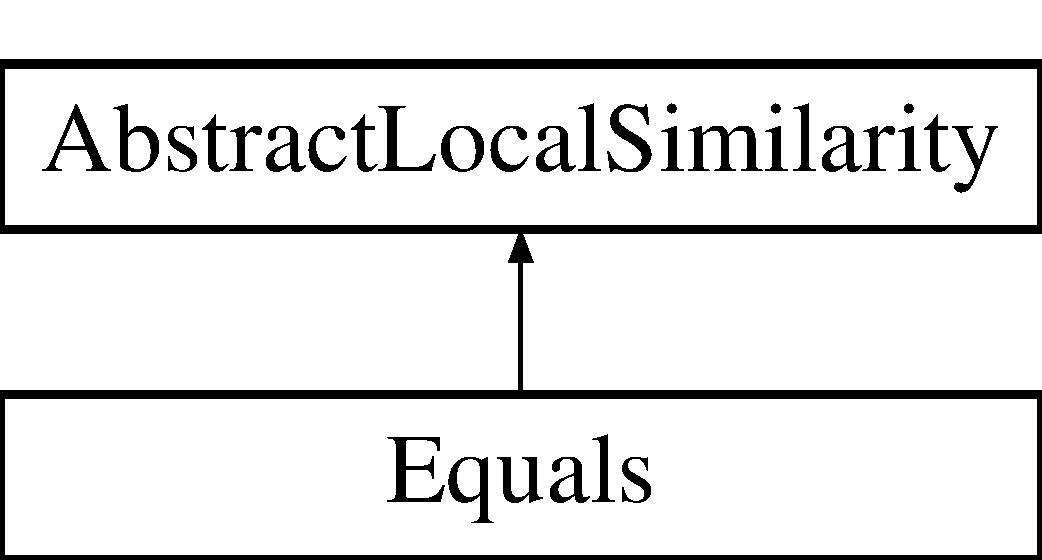
\includegraphics[height=2.000000cm]{class_equals}
\end{center}
\end{figure}
\subsection*{Public Member Functions}
\begin{DoxyCompactItemize}
\item 
\hyperlink{class_equals_a9ddef758a33b1c30e85a72b3c4db21fc}{Equals} ()
\begin{DoxyCompactList}\small\item\em Construtor da classe \hyperlink{class_equals}{Equals}. \end{DoxyCompactList}\item 
override float \hyperlink{class_equals_a1b7c994cee3bf4ff55f6eaef5f31c871}{Get\+Similarity} (\hyperlink{class_consult_params}{Consult\+Params} consult\+Params, \hyperlink{class_case}{Case} search\+Case, \hyperlink{class_case}{Case} retrieve\+Case)
\begin{DoxyCompactList}\small\item\em Método que retorna o valor de similaridade entre duas strings. \end{DoxyCompactList}\end{DoxyCompactItemize}


\subsection{Detailed Description}
Classe utilizada como função de similaridade local na qual compara se dois atributos são iguais. 



Definition at line 6 of file Equals.\+cs.



\subsection{Constructor \& Destructor Documentation}
\hypertarget{class_equals_a9ddef758a33b1c30e85a72b3c4db21fc}{}\label{class_equals_a9ddef758a33b1c30e85a72b3c4db21fc} 
\index{Equals@{Equals}!Equals@{Equals}}
\index{Equals@{Equals}!Equals@{Equals}}
\subsubsection{\texorpdfstring{Equals()}{Equals()}}
{\footnotesize\ttfamily Equals.\+Equals (\begin{DoxyParamCaption}{ }\end{DoxyParamCaption})}



Construtor da classe \hyperlink{class_equals}{Equals}. 



Definition at line 12 of file Equals.\+cs.



\subsection{Member Function Documentation}
\hypertarget{class_equals_a1b7c994cee3bf4ff55f6eaef5f31c871}{}\label{class_equals_a1b7c994cee3bf4ff55f6eaef5f31c871} 
\index{Equals@{Equals}!Get\+Similarity@{Get\+Similarity}}
\index{Get\+Similarity@{Get\+Similarity}!Equals@{Equals}}
\subsubsection{\texorpdfstring{Get\+Similarity()}{GetSimilarity()}}
{\footnotesize\ttfamily override float Equals.\+Get\+Similarity (\begin{DoxyParamCaption}\item[{\hyperlink{class_consult_params}{Consult\+Params}}]{consult\+Params,  }\item[{\hyperlink{class_case}{Case}}]{search\+Case,  }\item[{\hyperlink{class_case}{Case}}]{retrieve\+Case }\end{DoxyParamCaption})\hspace{0.3cm}{\ttfamily [virtual]}}



Método que retorna o valor de similaridade entre duas strings. 


\begin{DoxyParams}{Parameters}
{\em consult\+Params} & Parâmetros da consulta.\\
\hline
{\em search\+Case} & Caso utilizado como consulta.\\
\hline
{\em retrive\+Case} & Caso recuperado da base de casos.\\
\hline
\end{DoxyParams}
\begin{DoxyReturn}{Returns}
Valor de similaridade entre duas strings.
\end{DoxyReturn}


Implements \hyperlink{class_abstract_local_similarity_a6c51b1fe09e99d509da0d3634225ca36}{Abstract\+Local\+Similarity}.



Definition at line 24 of file Equals.\+cs.



The documentation for this class was generated from the following file\+:\begin{DoxyCompactItemize}
\item 
Similarity\+Measures/\+Local\+Similarities/\hyperlink{_equals_8cs}{Equals.\+cs}\end{DoxyCompactItemize}

\hypertarget{class_euclidean_distance}{}\section{Euclidean\+Distance Class Reference}
\label{class_euclidean_distance}\index{Euclidean\+Distance@{Euclidean\+Distance}}


Classe que utiliza da função da Distância Euclidiana para calcular a similaridade global entre dois casos.  


Inheritance diagram for Euclidean\+Distance\+:\begin{figure}[H]
\begin{center}
\leavevmode
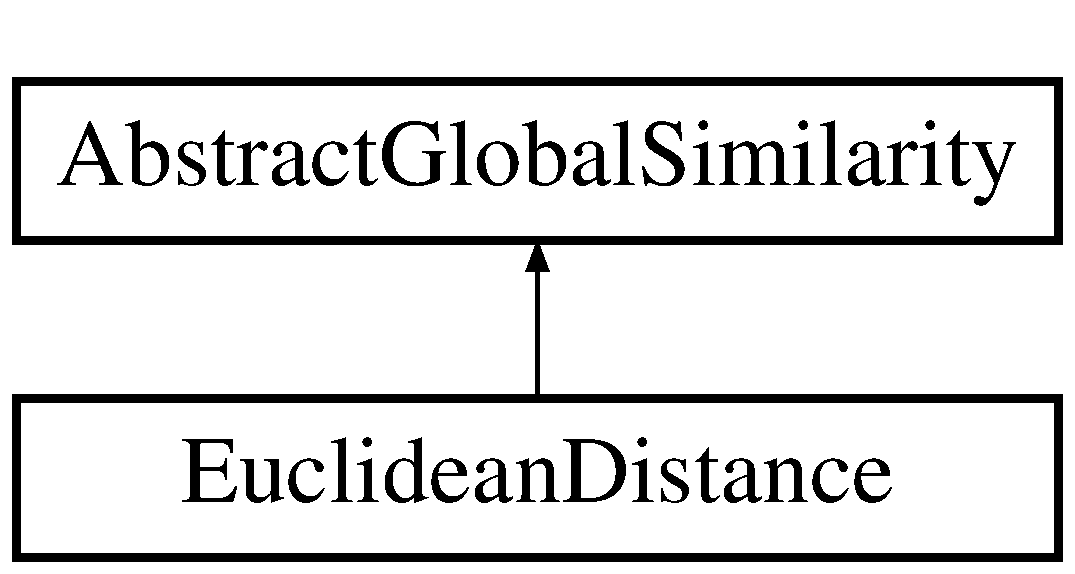
\includegraphics[height=2.000000cm]{class_euclidean_distance}
\end{center}
\end{figure}
\subsection*{Public Member Functions}
\begin{DoxyCompactItemize}
\item 
\hyperlink{class_euclidean_distance_aaa6a56ca6465502e28906a0c6b89318c}{Euclidean\+Distance} (\hyperlink{class_consult_structure}{Consult\+Structure} \hyperlink{class_abstract_global_similarity_a471ea41af416fd702d48f3b143416e66}{consult\+Structure})
\begin{DoxyCompactList}\small\item\em Construtor da classe \hyperlink{class_euclidean_distance}{Euclidean\+Distance}. \end{DoxyCompactList}\item 
override float \hyperlink{class_euclidean_distance_a1b27b1fd06df3e3defca37187634951e}{Get\+Similarity} (\hyperlink{class_case}{Case} search\+Case, \hyperlink{class_case}{Case} retrieve\+Case)
\begin{DoxyCompactList}\small\item\em Método que retorna o valor (entre 0 e 1) de similaridade entre dois casos utilizando a função da Distância Euclidiana. \end{DoxyCompactList}\end{DoxyCompactItemize}
\subsection*{Additional Inherited Members}


\subsection{Detailed Description}
Classe que utiliza da função da Distância Euclidiana para calcular a similaridade global entre dois casos. 



Definition at line 7 of file Euclidean\+Distance.\+cs.



\subsection{Constructor \& Destructor Documentation}
\hypertarget{class_euclidean_distance_aaa6a56ca6465502e28906a0c6b89318c}{}\label{class_euclidean_distance_aaa6a56ca6465502e28906a0c6b89318c} 
\index{Euclidean\+Distance@{Euclidean\+Distance}!Euclidean\+Distance@{Euclidean\+Distance}}
\index{Euclidean\+Distance@{Euclidean\+Distance}!Euclidean\+Distance@{Euclidean\+Distance}}
\subsubsection{\texorpdfstring{Euclidean\+Distance()}{EuclideanDistance()}}
{\footnotesize\ttfamily Euclidean\+Distance.\+Euclidean\+Distance (\begin{DoxyParamCaption}\item[{\hyperlink{class_consult_structure}{Consult\+Structure}}]{consult\+Structure }\end{DoxyParamCaption})}



Construtor da classe \hyperlink{class_euclidean_distance}{Euclidean\+Distance}. 


\begin{DoxyParams}{Parameters}
{\em consult\+Structure} & Estrutura de consulta que será utilizada na análise de similaridade.\\
\hline
\end{DoxyParams}


Definition at line 13 of file Euclidean\+Distance.\+cs.



\subsection{Member Function Documentation}
\hypertarget{class_euclidean_distance_a1b27b1fd06df3e3defca37187634951e}{}\label{class_euclidean_distance_a1b27b1fd06df3e3defca37187634951e} 
\index{Euclidean\+Distance@{Euclidean\+Distance}!Get\+Similarity@{Get\+Similarity}}
\index{Get\+Similarity@{Get\+Similarity}!Euclidean\+Distance@{Euclidean\+Distance}}
\subsubsection{\texorpdfstring{Get\+Similarity()}{GetSimilarity()}}
{\footnotesize\ttfamily override float Euclidean\+Distance.\+Get\+Similarity (\begin{DoxyParamCaption}\item[{\hyperlink{class_case}{Case}}]{search\+Case,  }\item[{\hyperlink{class_case}{Case}}]{retrieve\+Case }\end{DoxyParamCaption})\hspace{0.3cm}{\ttfamily [virtual]}}



Método que retorna o valor (entre 0 e 1) de similaridade entre dois casos utilizando a função da Distância Euclidiana. 


\begin{DoxyParams}{Parameters}
{\em search\+Case} & Caso utilizado como consulta.\\
\hline
{\em retrieve\+Case} & Casos recuperado da base de casos.\\
\hline
\end{DoxyParams}
\begin{DoxyReturn}{Returns}
Valor (entre 0 e 1) de similaridade entre dois casos
\end{DoxyReturn}


Implements \hyperlink{class_abstract_global_similarity_a4b97677ae2f5a0bdee41019b40b45114}{Abstract\+Global\+Similarity}.



Definition at line 24 of file Euclidean\+Distance.\+cs.



The documentation for this class was generated from the following file\+:\begin{DoxyCompactItemize}
\item 
Similarity\+Measures/\+Global\+Similarities/\hyperlink{_euclidean_distance_8cs}{Euclidean\+Distance.\+cs}\end{DoxyCompactItemize}

\hypertarget{class_linear_function}{}\section{Linear\+Function Class Reference}
\label{class_linear_function}\index{Linear\+Function@{Linear\+Function}}


Classe que utilizar uma função linear para calcular a similaridade local entre dois atributos do caso.  


Inheritance diagram for Linear\+Function\+:\begin{figure}[H]
\begin{center}
\leavevmode
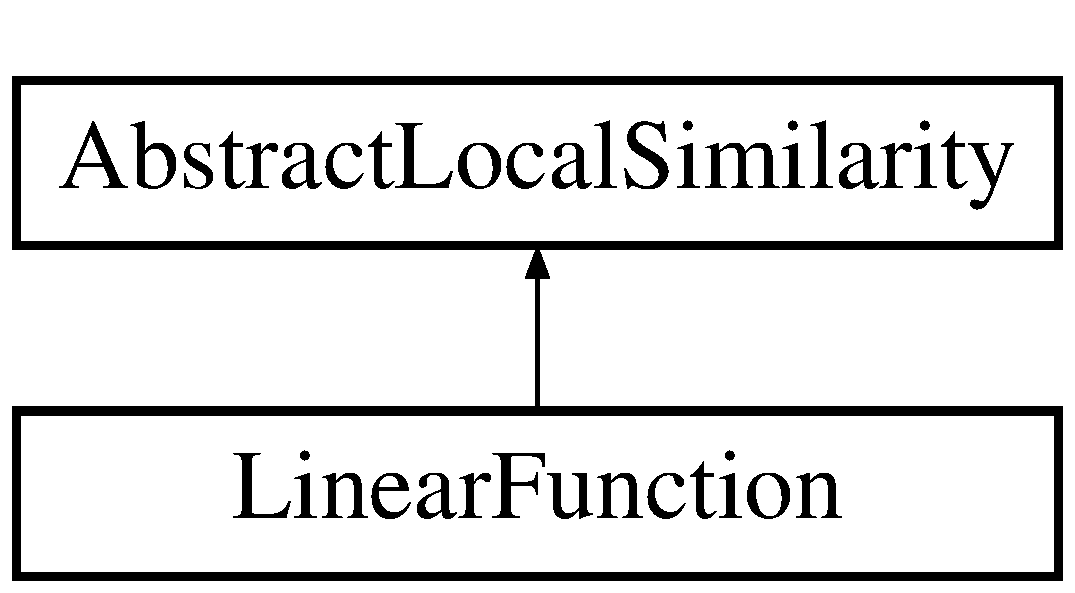
\includegraphics[height=2.000000cm]{class_linear_function}
\end{center}
\end{figure}
\subsection*{Public Member Functions}
\begin{DoxyCompactItemize}
\item 
\hyperlink{class_linear_function_ac8a3882badd498ea34c032d63aca3715}{Linear\+Function} (float min\+Val, float max\+Val)
\begin{DoxyCompactList}\small\item\em Construtor da classe \hyperlink{class_linear_function}{Linear\+Function}. \end{DoxyCompactList}\item 
override float \hyperlink{class_linear_function_addbfc2ff35037c40ae27c30e993e82ca}{Get\+Similarity} (\hyperlink{class_consult_params}{Consult\+Params} consult\+Params, \hyperlink{class_case}{Case} search\+Case, \hyperlink{class_case}{Case} retrive\+Case)
\begin{DoxyCompactList}\small\item\em Método que retorna o valor de similaridade entre dois números. \end{DoxyCompactList}\end{DoxyCompactItemize}


\subsection{Detailed Description}
Classe que utilizar uma função linear para calcular a similaridade local entre dois atributos do caso. 



Definition at line 7 of file Linear\+Function.\+cs.



\subsection{Constructor \& Destructor Documentation}
\hypertarget{class_linear_function_ac8a3882badd498ea34c032d63aca3715}{}\label{class_linear_function_ac8a3882badd498ea34c032d63aca3715} 
\index{Linear\+Function@{Linear\+Function}!Linear\+Function@{Linear\+Function}}
\index{Linear\+Function@{Linear\+Function}!Linear\+Function@{Linear\+Function}}
\subsubsection{\texorpdfstring{Linear\+Function()}{LinearFunction()}}
{\footnotesize\ttfamily Linear\+Function.\+Linear\+Function (\begin{DoxyParamCaption}\item[{float}]{min\+Val,  }\item[{float}]{max\+Val }\end{DoxyParamCaption})}



Construtor da classe \hyperlink{class_linear_function}{Linear\+Function}. 


\begin{DoxyParams}{Parameters}
{\em min\+Val} & Valor mínimo do domínio do atributo.\\
\hline
{\em max\+Val} & Valor máximo do domínio do atributo.\\
\hline
\end{DoxyParams}


Definition at line 24 of file Linear\+Function.\+cs.



\subsection{Member Function Documentation}
\hypertarget{class_linear_function_addbfc2ff35037c40ae27c30e993e82ca}{}\label{class_linear_function_addbfc2ff35037c40ae27c30e993e82ca} 
\index{Linear\+Function@{Linear\+Function}!Get\+Similarity@{Get\+Similarity}}
\index{Get\+Similarity@{Get\+Similarity}!Linear\+Function@{Linear\+Function}}
\subsubsection{\texorpdfstring{Get\+Similarity()}{GetSimilarity()}}
{\footnotesize\ttfamily override float Linear\+Function.\+Get\+Similarity (\begin{DoxyParamCaption}\item[{\hyperlink{class_consult_params}{Consult\+Params}}]{consult\+Params,  }\item[{\hyperlink{class_case}{Case}}]{search\+Case,  }\item[{\hyperlink{class_case}{Case}}]{retrive\+Case }\end{DoxyParamCaption})\hspace{0.3cm}{\ttfamily [virtual]}}



Método que retorna o valor de similaridade entre dois números. 


\begin{DoxyParams}{Parameters}
{\em consult\+Params} & Parâmetros da consulta.\\
\hline
{\em search\+Case} & Caso utilizado como consulta.\\
\hline
{\em retrive\+Case} & Caso recuperado da base de casos.\\
\hline
\end{DoxyParams}
\begin{DoxyReturn}{Returns}
Valor de similaridade entre dois números.
\end{DoxyReturn}


Implements \hyperlink{class_abstract_local_similarity_a6c51b1fe09e99d509da0d3634225ca36}{Abstract\+Local\+Similarity}.



Definition at line 37 of file Linear\+Function.\+cs.



The documentation for this class was generated from the following file\+:\begin{DoxyCompactItemize}
\item 
Similarity\+Measures/\+Local\+Similarities/\hyperlink{_linear_function_8cs}{Linear\+Function.\+cs}\end{DoxyCompactItemize}

\hypertarget{class_result}{}\section{Result Class Reference}
\label{class_result}\index{Result@{Result}}


Classe que representa o resultado da consulta realizada na biblioteca C\+BR.  


\subsection*{Public Member Functions}
\begin{DoxyCompactItemize}
\item 
\hyperlink{class_result_ac9674ce4ca5ac25deca347f06beb9b12}{Result} (int \hyperlink{class_result_ae4269cd3aa3565fa41da9ea75c364705}{id}, \hyperlink{class_case}{Case} \hyperlink{class_result_a715e03ca8c315d38e8e6842f3e6f710e}{match\+Case}, float \hyperlink{class_result_a591657b84ecc4e2b0c2f50e824a5c45a}{match\+Percentage})
\begin{DoxyCompactList}\small\item\em Construtor da classe \hyperlink{class_result}{Result}. \end{DoxyCompactList}\end{DoxyCompactItemize}
\subsection*{Public Attributes}
\begin{DoxyCompactItemize}
\item 
int \hyperlink{class_result_ae4269cd3aa3565fa41da9ea75c364705}{id}
\begin{DoxyCompactList}\small\item\em Identificador do resultado. \end{DoxyCompactList}\item 
\hyperlink{class_case}{Case} \hyperlink{class_result_a715e03ca8c315d38e8e6842f3e6f710e}{match\+Case}
\begin{DoxyCompactList}\small\item\em Caso da base de casos que foi comparado. \end{DoxyCompactList}\item 
float \hyperlink{class_result_a591657b84ecc4e2b0c2f50e824a5c45a}{match\+Percentage}
\begin{DoxyCompactList}\small\item\em Porcentagem de similaridade entre o caso de consulta e o caso da base de casos. \end{DoxyCompactList}\end{DoxyCompactItemize}


\subsection{Detailed Description}
Classe que representa o resultado da consulta realizada na biblioteca C\+BR. 



Definition at line 7 of file Result.\+cs.



\subsection{Constructor \& Destructor Documentation}
\hypertarget{class_result_ac9674ce4ca5ac25deca347f06beb9b12}{}\label{class_result_ac9674ce4ca5ac25deca347f06beb9b12} 
\index{Result@{Result}!Result@{Result}}
\index{Result@{Result}!Result@{Result}}
\subsubsection{\texorpdfstring{Result()}{Result()}}
{\footnotesize\ttfamily Result.\+Result (\begin{DoxyParamCaption}\item[{int}]{id,  }\item[{\hyperlink{class_case}{Case}}]{match\+Case,  }\item[{float}]{match\+Percentage }\end{DoxyParamCaption})}



Construtor da classe \hyperlink{class_result}{Result}. 


\begin{DoxyParams}{Parameters}
{\em id} & Identificador do resultado.\\
\hline
{\em match\+Case} & Caso da base de casos que foi comparado.\\
\hline
{\em match\+Percentage} & Porcentagem de similaridade entre o caso de consulta e o caso da base de casos.\\
\hline
\end{DoxyParams}


Definition at line 31 of file Result.\+cs.



\subsection{Member Data Documentation}
\hypertarget{class_result_ae4269cd3aa3565fa41da9ea75c364705}{}\label{class_result_ae4269cd3aa3565fa41da9ea75c364705} 
\index{Result@{Result}!id@{id}}
\index{id@{id}!Result@{Result}}
\subsubsection{\texorpdfstring{id}{id}}
{\footnotesize\ttfamily int Result.\+id}



Identificador do resultado. 



Definition at line 12 of file Result.\+cs.

\hypertarget{class_result_a715e03ca8c315d38e8e6842f3e6f710e}{}\label{class_result_a715e03ca8c315d38e8e6842f3e6f710e} 
\index{Result@{Result}!match\+Case@{match\+Case}}
\index{match\+Case@{match\+Case}!Result@{Result}}
\subsubsection{\texorpdfstring{match\+Case}{matchCase}}
{\footnotesize\ttfamily \hyperlink{class_case}{Case} Result.\+match\+Case}



Caso da base de casos que foi comparado. 



Definition at line 17 of file Result.\+cs.

\hypertarget{class_result_a591657b84ecc4e2b0c2f50e824a5c45a}{}\label{class_result_a591657b84ecc4e2b0c2f50e824a5c45a} 
\index{Result@{Result}!match\+Percentage@{match\+Percentage}}
\index{match\+Percentage@{match\+Percentage}!Result@{Result}}
\subsubsection{\texorpdfstring{match\+Percentage}{matchPercentage}}
{\footnotesize\ttfamily float Result.\+match\+Percentage}



Porcentagem de similaridade entre o caso de consulta e o caso da base de casos. 



Definition at line 22 of file Result.\+cs.



The documentation for this class was generated from the following file\+:\begin{DoxyCompactItemize}
\item 
Core/\hyperlink{_result_8cs}{Result.\+cs}\end{DoxyCompactItemize}

\hypertarget{class_search}{}\section{Search Class Reference}
\label{class_search}\index{Search@{Search}}


Classe responsável por realizar o matching entre o caso de consulta e todos os casos da base de casos.  


\subsection*{Public Member Functions}
\begin{DoxyCompactItemize}
\item 
\hyperlink{class_search_a1caef9f0a4ecf2b7ac8b75dd3b0175b2}{Search} ()
\begin{DoxyCompactList}\small\item\em Construtor da classe \hyperlink{class_search}{Search}. \end{DoxyCompactList}\item 
List$<$ \hyperlink{class_result}{Result} $>$ \hyperlink{class_search_ad64beea83d7d2a74950c327ec443daf9}{Do\+Search} (\hyperlink{class_case}{Case} search\+Case, \hyperlink{class_case_base_connector}{Case\+Base\+Connector} case\+Base\+Connector, \hyperlink{class_consult_structure}{Consult\+Structure} consult\+Structure)
\begin{DoxyCompactList}\small\item\em Realiza o matching entre o caso de consulta e o caso da base de casos e retorna o resultado desse matching. \end{DoxyCompactList}\end{DoxyCompactItemize}


\subsection{Detailed Description}
Classe responsável por realizar o matching entre o caso de consulta e todos os casos da base de casos. 



Definition at line 8 of file Search.\+cs.



\subsection{Constructor \& Destructor Documentation}
\hypertarget{class_search_a1caef9f0a4ecf2b7ac8b75dd3b0175b2}{}\label{class_search_a1caef9f0a4ecf2b7ac8b75dd3b0175b2} 
\index{Search@{Search}!Search@{Search}}
\index{Search@{Search}!Search@{Search}}
\subsubsection{\texorpdfstring{Search()}{Search()}}
{\footnotesize\ttfamily Search.\+Search (\begin{DoxyParamCaption}{ }\end{DoxyParamCaption})}



Construtor da classe \hyperlink{class_search}{Search}. 



Definition at line 13 of file Search.\+cs.



\subsection{Member Function Documentation}
\hypertarget{class_search_ad64beea83d7d2a74950c327ec443daf9}{}\label{class_search_ad64beea83d7d2a74950c327ec443daf9} 
\index{Search@{Search}!Do\+Search@{Do\+Search}}
\index{Do\+Search@{Do\+Search}!Search@{Search}}
\subsubsection{\texorpdfstring{Do\+Search()}{DoSearch()}}
{\footnotesize\ttfamily List$<$\hyperlink{class_result}{Result}$>$ Search.\+Do\+Search (\begin{DoxyParamCaption}\item[{\hyperlink{class_case}{Case}}]{search\+Case,  }\item[{\hyperlink{class_case_base_connector}{Case\+Base\+Connector}}]{case\+Base\+Connector,  }\item[{\hyperlink{class_consult_structure}{Consult\+Structure}}]{consult\+Structure }\end{DoxyParamCaption})}



Realiza o matching entre o caso de consulta e o caso da base de casos e retorna o resultado desse matching. 


\begin{DoxyParams}{Parameters}
{\em search\+Case} & Caso de consulta.\\
\hline
{\em case\+Base\+Connector} & Conector da base de casos.\\
\hline
{\em consult\+Structure} & Estrutura de consulta que será utilizada.\\
\hline
\end{DoxyParams}
\begin{DoxyReturn}{Returns}
Lista de \hyperlink{class_result}{Result} que contém o resultado de cada matching.
\end{DoxyReturn}


Definition at line 25 of file Search.\+cs.



The documentation for this class was generated from the following file\+:\begin{DoxyCompactItemize}
\item 
Core/\hyperlink{_search_8cs}{Search.\+cs}\end{DoxyCompactItemize}

\chapter{File Documentation}
\hypertarget{_abstract_feature_8cs}{}\section{Abstract\+Classes/\+Abstract\+Feature.cs File Reference}
\label{_abstract_feature_8cs}\index{Abstract\+Classes/\+Abstract\+Feature.\+cs@{Abstract\+Classes/\+Abstract\+Feature.\+cs}}
\subsection*{Classes}
\begin{DoxyCompactItemize}
\item 
class \hyperlink{class_abstract_feature}{Abstract\+Feature}
\begin{DoxyCompactList}\small\item\em Classe abstrata que representa a estrutura básica de um atributo. \end{DoxyCompactList}\end{DoxyCompactItemize}

\hypertarget{_abstract_global_similarity_8cs}{}\section{Abstract\+Classes/\+Abstract\+Global\+Similarity.cs File Reference}
\label{_abstract_global_similarity_8cs}\index{Abstract\+Classes/\+Abstract\+Global\+Similarity.\+cs@{Abstract\+Classes/\+Abstract\+Global\+Similarity.\+cs}}
\subsection*{Classes}
\begin{DoxyCompactItemize}
\item 
class \hyperlink{class_abstract_global_similarity}{Abstract\+Global\+Similarity}
\begin{DoxyCompactList}\small\item\em Classe abstrata que representa uma medida de similaridade global que será implementada na biblioteca C\+BR. \end{DoxyCompactList}\end{DoxyCompactItemize}

\hypertarget{_abstract_local_similarity_8cs}{}\section{Abstract\+Classes/\+Abstract\+Local\+Similarity.cs File Reference}
\label{_abstract_local_similarity_8cs}\index{Abstract\+Classes/\+Abstract\+Local\+Similarity.\+cs@{Abstract\+Classes/\+Abstract\+Local\+Similarity.\+cs}}
\subsection*{Classes}
\begin{DoxyCompactItemize}
\item 
class \hyperlink{class_abstract_local_similarity}{Abstract\+Local\+Similarity}
\begin{DoxyCompactList}\small\item\em Classe abstrata que representa uma medida de similaridade local que será implementada na biblioteca C\+BR. \end{DoxyCompactList}\end{DoxyCompactItemize}

\hypertarget{_case_8cs}{}\section{Core/\+Case.cs File Reference}
\label{_case_8cs}\index{Core/\+Case.\+cs@{Core/\+Case.\+cs}}
\subsection*{Classes}
\begin{DoxyCompactItemize}
\item 
class \hyperlink{class_case}{Case}
\begin{DoxyCompactList}\small\item\em Classe que representa um caso que compõem a base de casos. Composta por um identificador do caso e sua descrição do problema e solução. \end{DoxyCompactList}\end{DoxyCompactItemize}

\hypertarget{_case_base_connector_8cs}{}\section{Core/\+Case\+Base\+Connector.cs File Reference}
\label{_case_base_connector_8cs}\index{Core/\+Case\+Base\+Connector.\+cs@{Core/\+Case\+Base\+Connector.\+cs}}
\subsection*{Classes}
\begin{DoxyCompactItemize}
\item 
class \hyperlink{class_case_base_connector}{Case\+Base\+Connector}
\begin{DoxyCompactList}\small\item\em Classe resposável por fazer a conexão entre a biblioteca C\+BR e a base de casos. \end{DoxyCompactList}\end{DoxyCompactItemize}

\hypertarget{_case_feature_8cs}{}\section{Core/\+Case\+Feature.cs File Reference}
\label{_case_feature_8cs}\index{Core/\+Case\+Feature.\+cs@{Core/\+Case\+Feature.\+cs}}
\subsection*{Classes}
\begin{DoxyCompactItemize}
\item 
class \hyperlink{class_case_feature}{Case\+Feature}
\begin{DoxyCompactList}\small\item\em Classe que representa um atributo presente na descrição do problema ou solução de um caso. \end{DoxyCompactList}\end{DoxyCompactItemize}

\hypertarget{_c_b_r_a_p_i_8cs}{}\section{Core/\+C\+B\+R\+A\+PI.cs File Reference}
\label{_c_b_r_a_p_i_8cs}\index{Core/\+C\+B\+R\+A\+P\+I.\+cs@{Core/\+C\+B\+R\+A\+P\+I.\+cs}}
\subsection*{Classes}
\begin{DoxyCompactItemize}
\item 
class \hyperlink{class_c_b_r_a_p_i}{C\+B\+R\+A\+PI}
\begin{DoxyCompactList}\small\item\em Classe que deve ser instanciada para ser possível utilizar a biblioteca C\+BR. \end{DoxyCompactList}\end{DoxyCompactItemize}

\hypertarget{_consult_params_8cs}{}\section{Core/\+Consult\+Params.cs File Reference}
\label{_consult_params_8cs}\index{Core/\+Consult\+Params.\+cs@{Core/\+Consult\+Params.\+cs}}
\subsection*{Classes}
\begin{DoxyCompactItemize}
\item 
class \hyperlink{class_consult_params}{Consult\+Params}
\begin{DoxyCompactList}\small\item\em Classe que contém os parâmetros da consulta que serão utilizados para a análise de similaridade entre dois casos. \end{DoxyCompactList}\end{DoxyCompactItemize}

\hypertarget{_consult_structure_8cs}{}\section{Core/\+Consult\+Structure.cs File Reference}
\label{_consult_structure_8cs}\index{Core/\+Consult\+Structure.\+cs@{Core/\+Consult\+Structure.\+cs}}
\subsection*{Classes}
\begin{DoxyCompactItemize}
\item 
class \hyperlink{class_consult_structure}{Consult\+Structure}
\begin{DoxyCompactList}\small\item\em Classe que contém a estrutura de consulta que será utilizada na análise de similaridade entre os casos. \end{DoxyCompactList}\end{DoxyCompactItemize}

\hypertarget{_result_8cs}{}\section{Core/\+Result.cs File Reference}
\label{_result_8cs}\index{Core/\+Result.\+cs@{Core/\+Result.\+cs}}
\subsection*{Classes}
\begin{DoxyCompactItemize}
\item 
class \hyperlink{class_result}{Result}
\begin{DoxyCompactList}\small\item\em Classe que representa o resultado da consulta realizada na biblioteca C\+BR. \end{DoxyCompactList}\end{DoxyCompactItemize}

\hypertarget{_search_8cs}{}\section{Core/\+Search.cs File Reference}
\label{_search_8cs}\index{Core/\+Search.\+cs@{Core/\+Search.\+cs}}
\subsection*{Classes}
\begin{DoxyCompactItemize}
\item 
class \hyperlink{class_search}{Search}
\begin{DoxyCompactList}\small\item\em Classe responsável por realizar o matching entre o caso de consulta e todos os casos da base de casos. \end{DoxyCompactList}\end{DoxyCompactItemize}

\hypertarget{_euclidean_distance_8cs}{}\section{Similarity\+Measures/\+Global\+Similarities/\+Euclidean\+Distance.cs File Reference}
\label{_euclidean_distance_8cs}\index{Similarity\+Measures/\+Global\+Similarities/\+Euclidean\+Distance.\+cs@{Similarity\+Measures/\+Global\+Similarities/\+Euclidean\+Distance.\+cs}}
\subsection*{Classes}
\begin{DoxyCompactItemize}
\item 
class \hyperlink{class_euclidean_distance}{Euclidean\+Distance}
\begin{DoxyCompactList}\small\item\em Classe que utiliza da função da Distância Euclidiana para calcular a similaridade global entre dois casos. \end{DoxyCompactList}\end{DoxyCompactItemize}

\hypertarget{_equals_8cs}{}\section{Similarity\+Measures/\+Local\+Similarities/\+Equals.cs File Reference}
\label{_equals_8cs}\index{Similarity\+Measures/\+Local\+Similarities/\+Equals.\+cs@{Similarity\+Measures/\+Local\+Similarities/\+Equals.\+cs}}
\subsection*{Classes}
\begin{DoxyCompactItemize}
\item 
class \hyperlink{class_equals}{Equals}
\begin{DoxyCompactList}\small\item\em Classe utilizada como função de similaridade local na qual compara se dois atributos são iguais. \end{DoxyCompactList}\end{DoxyCompactItemize}

\hypertarget{_linear_function_8cs}{}\section{Similarity\+Measures/\+Local\+Similarities/\+Linear\+Function.cs File Reference}
\label{_linear_function_8cs}\index{Similarity\+Measures/\+Local\+Similarities/\+Linear\+Function.\+cs@{Similarity\+Measures/\+Local\+Similarities/\+Linear\+Function.\+cs}}
\subsection*{Classes}
\begin{DoxyCompactItemize}
\item 
class \hyperlink{class_linear_function}{Linear\+Function}
\begin{DoxyCompactList}\small\item\em Classe que utilizar uma função linear para calcular a similaridade local entre dois atributos do caso. \end{DoxyCompactList}\end{DoxyCompactItemize}

%--- End generated contents ---

% Index
\backmatter
\newpage
\phantomsection
\clearemptydoublepage
\addcontentsline{toc}{chapter}{Index}
\printindex

\end{document}
